\documentclass[notes,11pt, aspectratio=169, xcolor=table]{beamer}

\usepackage{pgfpages}
% These slides also contain speaker notes. You can print just the slides,
% just the notes, or both, depending on the setting below. Comment out the want
% you want.
\setbeameroption{hide notes} % Only slide
%\setbeameroption{show only notes} % Only notes
%\setbeameroption{show notes on second screen=right} % Both

\usepackage{helvet}
\usepackage[default]{lato}
\usepackage{array}
\usepackage{minted}

\newtheorem{proposition}{Proposition}

\usepackage{tikz}
\usetikzlibrary{shapes.geometric}
\usepackage{pgfplots}
\usepackage{graphicx}
\usepackage{verbatim}
\setbeamertemplate{note page}{\pagecolor{yellow!5}\insertnote}
\usetikzlibrary{positioning}
\usetikzlibrary{snakes}
\usetikzlibrary{calc}
\usetikzlibrary{arrows}
\usetikzlibrary{decorations.markings}
\usetikzlibrary{shapes.misc}
\usetikzlibrary{matrix,shapes,arrows,fit,tikzmark}
\usepackage{amsmath}
\usepackage{mathpazo}
\usepackage{hyperref}
\usepackage{lipsum}
\usepackage{multimedia}
\usepackage{graphicx}
\usepackage{multirow}
\usepackage{graphicx}
\usepackage{dcolumn}
\usepackage{bbm}
\usepackage[style=authoryear,sorting=nyt,uniquename=false]{biblatex}

\addbibresource{references.bib} 

\newcolumntype{d}[0]{D{.}{.}{5}}

\def\@@mybluebox[#1][#2]#3{
    \sbox\mytempbox{#3}%
    \mytemplen\ht\mytempbox
    \advance\mytemplen #1\relax
    \ht\mytempbox\mytemplen
    \mytemplen\dp\mytempbox
    \advance\mytemplen #2\relax
    \dp\mytempbox\mytemplen
    \colorbox{myblue}{\hspace{1em}\usebox{\mytempbox}\hspace{1em}}}


\usepackage{changepage}
\usepackage{appendixnumberbeamer}
\newcommand{\beginbackup}{
   \newcounter{framenumbervorappendix}
   \setcounter{framenumbervorappendix}{\value{framenumber}}
   \setbeamertemplate{footline}
   {
     \leavevmode%
     \hline
     box{%
       \begin{beamercolorbox}[wd=\paperwidth,ht=2.25ex,dp=1ex,right]{footlinecolor}%
%         \insertframenumber  \hspace*{2ex} 
       \end{beamercolorbox}}%
     \vskip0pt%
   }
 }
\newcommand{\backupend}{
   \addtocounter{framenumbervorappendix}{-\value{framenumber}}
   \addtocounter{framenumber}{\value{framenumbervorappendix}} 
}


\usepackage{graphicx}
\usepackage[space]{grffile}
\usepackage{booktabs}

% These are my colors -- there are many like them, but these ones are mine.
\definecolor{blue}{RGB}{0,114,178}
\definecolor{red}{RGB}{213,94,0}
\definecolor{yellow}{RGB}{240,228,66}
\definecolor{green}{RGB}{0,158,115}
\newcommand{\blue}[1]{\textcolor{blue}{#1}}

\hypersetup{
  colorlinks=false,
  linkbordercolor = {white},
  linkcolor = {blue}
}


%% I use a beige off white for my background
\definecolor{MyBackground}{RGB}{255,253,218}

%% Uncomment this if you want to change the background color to something else
%\setbeamercolor{background canvas}{bg=MyBackground}

%% Change the bg color to adjust your transition slide background color!
\newenvironment{transitionframe}{
  \setbeamercolor{background canvas}{bg=yellow}
  \begin{frame}}{
    \end{frame}
}

\setbeamercolor{frametitle}{fg=blue}
\setbeamercolor{title}{fg=blue}
\setbeamertemplate{footline}[frame number]
\setbeamertemplate{navigation symbols}{} 
\setbeamertemplate{itemize items}{-}
\setbeamercolor{itemize item}{fg=blue}
\setbeamercolor{itemize subitem}{fg=blue}
\setbeamercolor{enumerate item}{fg=blue}
\setbeamercolor{enumerate subitem}{fg=blue}
\setbeamercolor{button}{bg=MyBackground,fg=blue,}



% If you like road maps, rather than having clutter at the top, have a roadmap show up at the end of each section 
% (and after your introduction)
% Uncomment this is if you want the roadmap!
% \AtBeginSection[]
% {
%    \begin{frame}
%        \frametitle{Roadmap of Talk}
%        \tableofcontents[currentsection]
%    \end{frame}
% }
\setbeamercolor{section in toc}{fg=blue}
\setbeamercolor{subsection in toc}{fg=red}
\setbeamersize{text margin left=1em,text margin right=1em} 

\newenvironment{wideitemize}{\itemize\addtolength{\itemsep}{10pt}}{\enditemize}

\usepackage{environ}
\NewEnviron{videoframe}[1]{
  \begin{frame}
    \vspace{-8pt}
    \begin{columns}[onlytextwidth, T] % align columns
      \begin{column}{.58\textwidth}
        \begin{minipage}[t][\textheight][t]
          {\dimexpr\textwidth}
          \vspace{8pt}
          \hspace{4pt} {\Large \sc \textcolor{blue}{#1}}
          \vspace{8pt}
          
          \BODY
        \end{minipage}
      \end{column}%
      \hfill%
      \begin{column}{.42\textwidth}
        \colorbox{green!20}{\begin{minipage}[t][1.2\textheight][t]
            {\dimexpr\textwidth}
            Face goes here
          \end{minipage}}
      \end{column}%
    \end{columns}
  \end{frame}
}

\title[]{International Trade: Review}
\subtitle[]{Midterm}
\author[Góes]
{Carlos Góes\inst{1}}
\date{Fall 2025}
\institute[GWU]{\inst{1} George Washington University }



\begin{document}

%%% TIKZ STUFF
\tikzset{   
        every picture/.style={remember picture,baseline},
        every node/.style={anchor=base,align=center,outer sep=1.5pt},
        every path/.style={thick},
        }
\newcommand\marktopleft[1]{%
    \tikz[overlay,remember picture] 
        \node (marker-#1-a) at (-.3em,.3em) {};%
}
\newcommand\markbottomright[2]{%
    \tikz[overlay,remember picture] 
        \node (marker-#1-b) at (0em,0em) {};%
}
\tikzstyle{every picture}+=[remember picture] 
\tikzstyle{mybox} =[draw=black, very thick, rectangle, inner sep=10pt, inner ysep=20pt]
\tikzstyle{fancytitle} =[draw=black,fill=red, text=white]
%%%% END TIKZ STUFF



%----------------------------------------------------------------------%
%-------------------       TITLE PAGE       ---------------------------%
%----------------------------------------------------------------------%





%----------------------------------------------------------------------%






%----------------------------------------------------------------------%
%----------------------------------------------------------------------%

%----------------------------------------------------------------------%
\frame{\titlepage}
\addtocounter{framenumber}{-1}
%----------------------------------------------------------------------%



%----------------------------------------------------------------------%
%----------------------------------------------------------------------%


\begin{frame}{Why do we trade?}
\begin{wideitemize}
    \item Have you engaged in trade today?
    \begin{itemize}
        \item You all are trading your future (hopefully higher) income for my teaching;
        \item I am teaching so that I can pay for my wife's handbags;
    \end{itemize}
    \item What makes countries (or people) trade?
    \vspace{12pt}

    \begin{itemize}
        \item Different skills (e.g., I am bad mechanic, so I pay Jiffy Lube instead)
        \item Different endowments (e.g., Saudi Arabia has a lot of oil; Luxembourg does not);
        \item Different products (e.g., both France and Italy produce wine, but trade for variety);
    \end{itemize}

\end{wideitemize}    
\end{frame}


\section{The principle of comparative advantage}

\begin{frame}{The principle of comparative advantage}
    \begin{wideitemize} 
        \item What we described above is the \textcolor{blue}{principle of comparative advantage}
        \item Countries/households will be better off by specializing in subset of activities + trading
    \end{wideitemize}
\vspace{24pt}
        \Huge
        \centering
        we call these \textcolor{blue}{gains from trade}
        \normalsize
\end{frame}

\begin{frame}
\addtocounter{framenumber}{-1}

\centering

\Huge{\blue{Classic Ricardian Model}}
    
\end{frame}

\section{Ricardian Model}

\begin{frame}{Ricardian Model: Preliminaries}
\begin{wideitemize}
        \item Consider a world with 2 countries (US, Colombia) and 2 products (Computers, Roses)
        \item Set of countries $i \in \{ US, COL\}$; set of products $p \in \{ C, R\}$
        \item In country $i$, there are $L_i$ units of labor (worker-hours) available 
        \item In country $i$, to produce one unit of good $p$, firms use $a_{i,p}$ units of labor
        \item $Y_{i,p}$ is total production of good $p$ in $i$
        \item To produce $Y_{i,C}$ units of computers in $i$, firms use $a_{i,C} \times Y_{i,C}$ units of labor 
        \item We call $a_{i,p}$ the \textbf{unit labor requirements}
        \begin{itemize}
            \item The higher $a_{i,p}$, the \textbf{less productive} country $i$ is in producing $p$. Why?
        \end{itemize}
        \item Consumers have preferences over both goods: $U_i(Q_{i,C},Q_{i,R}) = Q_{i,C}^{\alpha_i} Q_{i,R}^{1-\alpha_i}$
        \item Trade is balanced
    \end{wideitemize}
\end{frame}


\begin{frame}{Production Possibilities Frontier}
\begin{wideitemize}
        \item Total labor can be distributed for the production of either good, such that:

        \begin{equation*}
            \underbrace{a_{i,C} \times Y_{i,C}}_{\substack{\text{labor used in} \\ \text{production of } C}} + \underbrace{a_{i,R} \times Y_{i,R}}_{\substack{\text{labor used in} \\ \text{production of } R}} \le \underbrace{L_i}_{\substack{\text{total labor} \\ \text{available in } i}}
        \end{equation*}

        \item English: if labor used to produce $(Y_{i,C}, Y_{i,R})$ is not larger than $L_i$, production is feasible
    \end{wideitemize}
\end{frame}


\begin{frame}{Production Possibilities Frontier, Graphical Example}

\begin{center}

\begin{figure}[htbp]

\begin{tikzpicture}
\begin{axis}[
    xlabel={Quantity of roses, $Y_{US,R}$},
    ylabel={Quantity of computers, $Y_{US,C}$},
    xmin=0, xmax=11,
    ymin=0, ymax=0.11,
    yticklabel=\empty,
    xticklabel=\empty,
    axis lines=left,
    enlargelimits=false,
    clip=false,
    axis on top,
    scaled x ticks=false,
    width=9cm, height=7cm,
    title={US},
    title style={font=\bfseries}
]

% Filled triangle under the PPF
\addplot [
    name path=A,
    domain=0:0.1,
    draw=none
] {.1 - 1/100*x};

\path[name path=B] (axis cs:0,0) -- (axis cs:10,0);

\addplot [
    fill=cyan!20,
    draw=none
] fill between [of=A and B];

% PPF line
\addplot[thick, blue, domain=0:10] {.1 - 1/100*x};

% Labels
\node at (axis cs:3.5,0.03) {\Large $\mathcal{Y}_{US}$};
\node at (axis cs:10,-.01) {\scriptsize $\frac{L_{US}}{a_{US,R}}$};
\node at (axis cs:-.75,.1) {\scriptsize $\frac{L_{US}}{a_{US,C}}$};
\node at (axis cs:10,0.05) { $\textcolor{blue}{Y_{US,C} = \frac{L_{US}}{a_{US,C}} - \frac{a_{US,R}}{a_{US,C}} \times Y_{US,R}}$};
\node at (axis cs:7,0.07) {\scriptsize \textcolor{blue}{Slope: opportunity cost} };

\end{axis}

\end{tikzpicture}

\end{figure}
\end{center}


\end{frame}


\begin{frame}{Production Technology}
\begin{wideitemize}
        \item In country $i$, firms producing good $p$ maximize profits under perfect competition:
        \begin{equation*}
            \max_{Y_{i,p}} \pi_{i,p} = \max_{Y_{i,p}} P_{i,p}Y_{i,p} - w_i a_{i,p} Y_{i,p} 
        \end{equation*}
        \item<2-> Since labor only one type of labor (mobile across sectors), there is a single wage $w_i$
        \item<3-> In equilibrium, \textbf{prices equal marginal cost} in each productive sector:
        \begin{eqnarray*}
            P_{i,p} = w_i a_{i,p} \iff \frac{P_{i,p}}{a_{i,p}} = w_i  \qquad \text{ for } p \in\{C,R\}
        \end{eqnarray*}
        \item<4-> We can pin down the relative price $P_{i,C} / P_{i,R}$:
        \begin{equation*}
            \frac{P_{i,C}}{a_{i,C}} = w_i = \frac{P_{i,R}}{a_{i,R}} \iff \frac{P_{i,C}}{P_{i,R}} = \frac{a_{i,C}}{a_{i,R}}  
        \end{equation*}
    \item<5-> In autarky, relative prices will reflect the \textbf{opportunity cost} within country $i$
    \end{wideitemize}
\end{frame}


\begin{frame}{Production Possibilities Frontier, Graphical Example}

\begin{center}

\begin{figure}[htbp]

\begin{tikzpicture}

\begin{axis}[
    xlabel={Quantity of roses, $Y_{US,R}$},
    ylabel={Quantity of computers, $Y_{US,C}$},
    xmin=0, xmax=11,
    ymin=0, ymax=0.11,
    yticklabel=\empty,
    xticklabel=\empty,
    axis lines=left,
    enlargelimits=false,
    clip=false,
    axis on top,
    scaled x ticks=false,
    width=9cm, height=7cm,
    title={US},
    title style={font=\bfseries}
]

% Filled triangle under the PPF
\addplot [
    name path=A,
    domain=0:0.1,
    draw=none
] {.1 - 1/100*x};

\path[name path=B] (axis cs:0,0) -- (axis cs:10,0);

\addplot [
    fill=cyan!20,
    draw=none
] fill between [of=A and B];

% PPF line
\addplot[thick, blue, domain=0:10] {.1 - 1/100*x};

% Labels
\node at (axis cs:3.5,0.03) {\Large $\mathcal{Y}_{US}$};
\node at (axis cs:10,-.01) {\scriptsize $\frac{L_{US}}{a_{US,R}}$};
\node at (axis cs:-.75,.1) {\scriptsize $\frac{L_{US}}{a_{US,C}}$};
\node at (axis cs:10,0.05) { $\textcolor{blue}{Y_{US,C} = \frac{L_{US}}{a_{US,C}} -} \textcolor{red}{ \frac{P_{US,R}}{P_{US,C}} } \textcolor{blue}{ \times Y_{US,R}}$};
\node at (axis cs:10,0.07) {\scriptsize \textcolor{red}{Slope = - 1/100: opportunity cost = relative prices} };



\end{axis}

\end{tikzpicture}

\end{figure}
\end{center}
\end{frame}


\begin{frame}{Preferences}
\begin{wideitemize}
        \item In country $i$, consumers preferences over products $p$, represented by a utility function. 

        \begin{equation*}
            U_i(Q_C,Q_R) \equiv Q_C^{\alpha_i} Q_R^{1-\alpha_i}, \qquad \text{for } 0 < \alpha_i < 1   
        \end{equation*}
        \item Consumers take prices $P_{i,R},P_{i,C}$ as given and maximize: 
        \begin{equation*}
            \max_{\{Q_{i,C}, Q_{i,R}\}} U_i(Q_{i,C}, Q_{i,R}) \equiv Q_{i,C}^{\alpha_i} Q_{i,R}^{1-\alpha_i} \qquad s.t. \qquad P_{i,C} Q_{i,C} + P_{i,R} Q_{i,R} = w_i L_i
        \end{equation*}
        \item How to solve this?
        \end{wideitemize}
\end{frame}

\begin{frame}{Preferences}
\begin{wideitemize}
        \item Rewrite budget constraint: $Q_{i,R} = \frac{w_i L_i}{P_{i,R}} - \frac{P_{i,C}}{P_{i,R} } Q_{i,C}$
        \item Replace in objective function and solve unconstrained max problem:

        \begin{equation*}
            \max_{\{Q_{i,C} \}} Q_C^{\alpha_i} \left( \frac{w_i L_i}{P_{i,R}} - \frac{P_{i,C}}{P_{i,R} } Q_{i,C} \right)^{1-\alpha_i}
        \end{equation*}
        \item First order condition: 
\scriptsize{
\begin{eqnarray*}
    & & \alpha_i Q_{i,C}^{\alpha_i-1} \left( \underbrace{\frac{w_i L_i}{P_{i,R}} - \frac{P_{i,C}}{P_{i,R} } Q_{i,C}}_{=Q_{i,R}} \right)^{1-\alpha_i} + Q_{i,C}^{\alpha_i} (1-\alpha_i) \left( \underbrace{\frac{w_i L_i}{P_{i,R}} - \frac{P_{i,C}}{P_{i,R} } Q_{i,C}}_{=Q_{i,R}} \right)^{1-\alpha_i-1} \left( - \frac{P_{i,C}}{P_{i,R}}\right) = 0 \\
%    & & \alpha_i  \left( \frac{Q_{i,R}}{Q_{i,C}} \right)^{1-\alpha_i} - (1-\alpha_i) \left( \frac{Q_{i,R}}{Q_{i,C}} \right)^{-\alpha_i} \left( \frac{P_{i,C}}{P_{i,R}}\right) = 0 \\
%    & & \alpha_i  \left( \frac{Q_{i,R}}{Q_{i,C}} \right)^{1-\alpha_i} = (1-\alpha_i) \left( \frac{Q_{i,R}}{Q_{i,C}} \right)^{-\alpha_i} \left( \frac{P_{i,C}}{P_{i,R}}\right) \\
%    & & \frac{Q_{i,R}}{Q_{i,C}}  = \frac{1-\alpha_i}{\alpha_i } \left( \frac{P_{i,C}}{P_{i,R}}\right) \\
\end{eqnarray*}
}
\normalsize
\begin{center}
    \boxed{$Q_{i,R}  = \frac{1-\alpha_i}{\alpha_i } \left( \frac{P_{i,C}}{P_{i,R}}\right) Q_{i,C}$}    
\end{center}

        \end{wideitemize}
\end{frame}

\begin{frame}{Preferences}
\begin{wideitemize}
        \item Replace result in budget constraint:

\scriptsize{
\begin{eqnarray*}
    Q_{i,R}&=& \frac{1-\alpha_i}{\alpha_i } \left( \frac{P_{i,C}}{P_{i,R}}\right) Q_{i,C}  = \frac{w_i L_i}{P_{i,R}} - \frac{P_{i,C}}{P_{i,R} } Q_{i,C} \\
    %\frac{1-\alpha_i}{\alpha_i } \left( \frac{P_{i,C}}{P_{i,R}}\right) Q_{i,C}  &=& \frac{w_i L_i}{P_{i,R}} - \frac{P_{i,C}}{P_{i,R} } Q_{i,C} \\
%    \frac{1-\alpha_i}{\alpha_i } \left( \frac{P_{i,C}}{P_{i,R}}\right) Q_{i,C} + \frac{P_{i,C}}{P_{i,R} } Q_{i,C} &=& \frac{w_i L_i}{P_{i,R}}  \\
%    \frac{1-\alpha_i + \alpha_i}{\alpha_i } \left( \frac{P_{i,C}}{P_{i,R}}\right) Q_{i,C} &=& \frac{w_i L_i}{P_{i,R}}  \\
\end{eqnarray*}
}

\normalsize
\begin{center}
    \boxed{$Q_{i,C} = \alpha_i  \frac{w_i L_i}{P_{i,C}}$}    
\end{center}


\item Finally:
{\scriptsize
\begin{eqnarray*}
     Q_{i,R}  &=& \frac{1-\alpha_i}{\alpha_i } \left( \frac{P_{i,C}}{P_{i,R}}\right) Q_{i,C}  = \frac{1-\alpha_i}{\alpha_i } \left( \frac{P_{i,C}}{P_{i,R}}\right) \alpha_i  \frac{w_i L_i}{P_{i,C}} \\
\end{eqnarray*}
}

\begin{center}
    \boxed{$Q_{i,R}  = (1-\alpha_i) \frac{w_i L_i}{P_{i,R}}$}    
\end{center}

\item Cobb-Douglas preferences: demand is a fixed share of their income $(\alpha_i, 1-\alpha_i)$; demand inversely proportional to the price of that good.
\item Holds regardless of whether consumers are in autarky or trade. 

\end{wideitemize}
\end{frame}

\begin{frame}{Prices in Autarky Equilibrium}
\begin{wideitemize}
        \item In equilibrium, \textbf{prices equal marginal cost} in each productive sector:
        \begin{eqnarray*}
            P_{i,p} = w_i a_{i,p} \iff \frac{P_{i,p}}{a_{i,p}} = w_i  \qquad \text{ for } p \in\{C,R\}
        \end{eqnarray*}
        \item<2-> In autarky equilibrium, there demand and production in both sectors
        \item We can pin down the relative price $P_{i,C} / P_{i,R}$:
        \begin{center}
        \boxed{
            \frac{P_{i,C}}{a_{i,C}} = w_i = \frac{P_{i,R}}{a_{i,R}} \iff \frac{P_{i,C}}{P_{i,R}} = \frac{a_{i,C}}{a_{i,R}}  
        }            
        \end{center}
    \item<3-> In autarky, relative prices will reflect the \textbf{opportunity cost} within country $i$

\end{wideitemize}
\end{frame}

\begin{frame}{Autarky Equilibrium}
\begin{wideitemize}
    \item Replacing $\frac{P_{i,p}}{a_{i,p}} = w_i \iff P_{i,C} = w_i a_{i,p}$ in demand functions solves in terms of parameters:
\begin{center}
    \boxed{$Q_{i,C} = \alpha_i  \frac{w_i L_i}{P_{i,C}}=  \alpha_i  \frac{L_i}{a_{i,C}} ,\qquad Q_{i,R}  = (1-\alpha_i) \frac{w_i L_i}{P_{i,R}} = (1-\alpha_i) \frac{L_i}{a_{i,R}}$}    
\end{center}
    \item<2-> In equilibrium, \blue{supply equals demand}:

    \begin{center}
    \boxed{$Y_{i,C} = Q_{i,C},\qquad Y_{i,R} = Q_{i,R}$}    
\end{center}

    \item<4-> We have solved for optimal demands $( Q_{i,C}, Q_{i,R})$, get $(Y_{i,C}, Y_{i,R})$   ``for free''
    \item<5->  Can check choices satisfy the PPF:
    {\scriptsize
        \begin{eqnarray*}
            a_{i,C} \times Y_{i,C} + a_{i,R} \times Y_{i,R} &=& L_i \\
            a_{i,C} \times Q_{i,C} + a_{i,R} \times Q_{i,R} &=& L_i \qquad (\text{mkt clearing}) \\
            a_{i,C} \times \alpha_i  \frac{L_i}{a_{i,C}} + a_{i,R} \times (1-\alpha_i) \frac{L_i}{a_{i,R}}  &=& L_i \qquad (\text{optimal demand}) \\
            \alpha_i  L_i + (1-\alpha_i) L_i  &=& L_i \qquad (\text{checks out!})
        \end{eqnarray*}
        }
\end{wideitemize}
\end{frame}

\begin{frame}{Numerical example: Autarky}
\centering
\resizebox{\textwidth}{!}{%
\begin{tabular}{lcc}
\toprule
\textbf{Variable} & \textbf{United States (US)} & \textbf{Colombia (COL)} \\
\midrule
Labor endowment $L_i$ & $300$ million & $54$ million \\
Preference parameter $\alpha_i$ & $1/2$ & $3/4$ \\
Unit labor requirement for computers $a_{i,C}$ & $3{,}000$ & $5{,}400$ \\
Unit labor requirement for roses $a_{i,R}$ & $30$ & $6$ \\
\midrule
Max computers: $L_i / a_{i,C}$ & \white{$300\text{m}/3{,}000 = 100{,}000$} & \white{$54\text{m}/5{,}400 = 10{,}000$} \\
Max roses: $L_i / a_{i,R}$ & \white{$300\text{m}/30 = 10\text{m}$} & \white{$54\text{m}/6 = 9\text{m}$} \\
\midrule
Opportunity cost $a_{i,C}/a_{i,R}$ & \white{$3{,}000/30 = 100$} & \white{$5{,}400/6 = 900$} \\
Demand for computers: $\alpha_i L_i / a_{i,C}$ & \white{$0.5 \times 300\text{m}/3{,}000 = 50{,}000$} & \white{$0.75 \times 54\text{m}/5{,}400 = 7{,}500$} \\
Demand for roses: $(1{-}\alpha_i) L_i / a_{i,R}$ & \white{$0.5 \times 300\text{m}/30 = 5\text{m}$} & \white{$0.25 \times 54\text{m}/6 = 2.25\text{m}$} \\
\bottomrule
\end{tabular}
}
\end{frame}

\begin{frame}{Numerical example: Autarky}
\addtocounter{framenumber}{-1}

\centering
\resizebox{\textwidth}{!}{%
\begin{tabular}{lcc}
\toprule
\textbf{Variable} & \textbf{United States (US)} & \textbf{Colombia (COL)} \\
\midrule
Labor endowment $L_i$ & $300$ million & $54$ million \\
Preference parameter $\alpha_i$ & $1/2$ & $3/4$ \\
Unit labor requirement for computers $a_{i,C}$ & $3{,}000$ & $5{,}400$ \\
Unit labor requirement for roses $a_{i,R}$ & $30$ & $6$ \\
\midrule
Max computers: $L_i / a_{i,C}$ & $300\text{m}/3{,}000 = 100{,}000$ & $54\text{m}/5{,}400 = 10{,}000$ \\
Max roses: $L_i / a_{i,R}$ & $300\text{m}/30 = 10\text{m}$ & $54\text{m}/6 = 9\text{m}$ \\
\midrule
Opportunity cost $a_{i,C}/a_{i,R}$ & \white{$3{,}000/30 = 100$} & \white{$5{,}400/6 = 900$} \\
Demand for computers: $\alpha_i L_i / a_{i,C}$ & \white{$0.5 \times 300\text{m}/3{,}000 = 50{,}000$} & \white{$0.75 \times 54\text{m}/5{,}400 = 7{,}500$} \\
Demand for roses: $(1{-}\alpha_i) L_i / a_{i,R}$ & \white{$0.5 \times 300\text{m}/30 = 5\text{m}$} & \white{$0.25 \times 54\text{m}/6 = 2.25\text{m}$} \\
\bottomrule
\end{tabular}
}
\end{frame}

\begin{frame}{Numerical example: Autarky}
\addtocounter{framenumber}{-1}
\centering
\resizebox{\textwidth}{!}{%
\begin{tabular}{lcc}
\toprule
\textbf{Variable} & \textbf{United States (US)} & \textbf{Colombia (COL)} \\
\midrule
Labor endowment $L_i$ & $300$ million & $54$ million \\
Preference parameter $\alpha_i$ & $1/2$ & $3/4$ \\
Unit labor requirement for computers $a_{i,C}$ & $3{,}000$ & $5{,}400$ \\
Unit labor requirement for roses $a_{i,R}$ & $30$ & $6$ \\
\midrule
Max computers: $L_i / a_{i,C}$ & $300\text{m}/3{,}000 = 100{,}000$ & $54\text{m}/5{,}400 = 10{,}000$ \\
Max roses: $L_i / a_{i,R}$ & $300\text{m}/30 = 10\text{m}$ & $54\text{m}/6 = 9\text{m}$ \\
\midrule
Opportunity cost $a_{i,C}/a_{i,R}$ & $3{,}000/30 = 100$ & $5{,}400/6 = 900$ \\
Demand for computers: $\alpha_i L_i / a_{i,C}$ & $0.5 \times 300\text{m}/3{,}000 = 50{,}000$ & $0.75 \times 54\text{m}/5{,}400 = 7{,}500$ \\
Demand for roses: $(1{-}\alpha_i) L_i / a_{i,R}$ & $0.5 \times 300\text{m}/30 = 5\text{m}$ & $0.25 \times 54\text{m}/6 = 2.25\text{m}$ \\
\bottomrule
\end{tabular}
}
\end{frame}

\begin{frame}{Autarky Equilibrium}
\begin{figure}[htbp!]

% California
\begin{subfigure}{}
\resizebox{0.48\textwidth}{!}{%
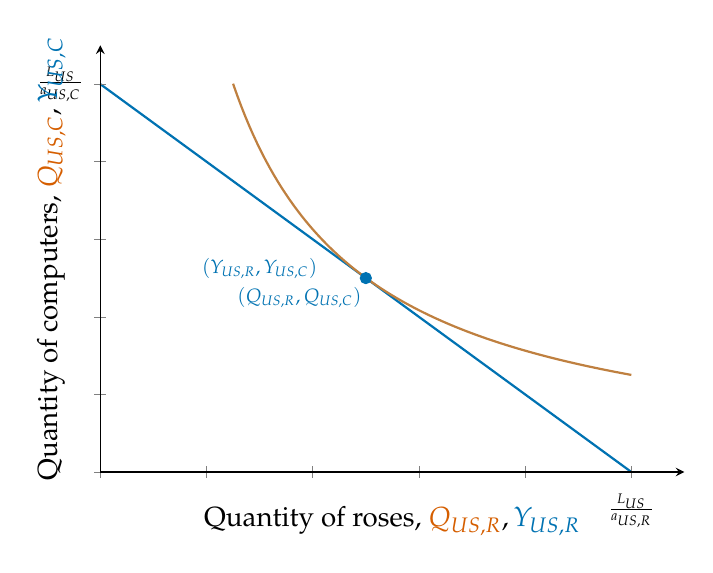
\begin{tikzpicture}
\pgfmathsetmacro{\aC}{100}       % unit labor requirement for computers
\pgfmathsetmacro{\aR}{1}         % unit labor requirement for roses
\pgfmathsetmacro{\alpha}{0.5}    % preference for computers
\pgfmathsetmacro{\Lendow}{10}    % labor endowment

% Compute equilibrium quantities
\pgfmathsetmacro{\Qc}{(\alpha*\Lendow)/\aC}
\pgfmathsetmacro{\Qr}{((1 - \alpha)*\Lendow)/\aR}

% Compute utility level
\pgfmathsetmacro{\U}{(\Qc^(\alpha))*(\Qr^(1 - \alpha))}

% Compute prefactor for indifference curve: Qc = A * Qr^(- (1 - alpha)/alpha)
\pgfmathsetmacro{\expo}{(1 - \alpha)/\alpha}
\pgfmathsetmacro{\A}{\U^(1/\alpha)}

\centering
\begin{axis}[
    ylabel={Quantity of computers, $\textcolor{red}{Q_{US,C}}, \textcolor{blue}{Y_{US,C}}$},
    xlabel={Quantity of roses, $\textcolor{red}{Q_{US,R}}, \textcolor{blue}{Y_{US,R}}$},
    ymin=0, ymax=0.11,
    xmin=0, xmax=11,
    yticklabel=\empty,
    xticklabel=\empty,
    axis lines=left,
    enlargelimits=false,
    clip=false,
    axis on top,
    scaled x ticks=false,
    width=9cm, height=7cm,
    title style={font=\bfseries}
]

% PPF: Q_C = (L/a_C) - (a_R/a_C) * Q_R
\addplot[thick, blue, domain=0:10] {\Lendow/\aC - (\aR/\aC)*x};

% Indifference curve through optimal bundle
\addplot[thick, brown, domain=2.5:10, samples=100] {\A * x^(-\expo)};

% Labels
%\node at (axis cs:3.5,0.03) {\Large $\mathcal{Y}_{US}$};
\node at (axis cs:\Lendow/\aR,-.01) {\scriptsize $\frac{L_{US}}{a_{US,R}}$};
\node at (axis cs:-.75,\Lendow/\aC) {\scriptsize $\frac{L_{US}}{a_{US,C}}$};


% Equilibrium point
\addplot[only marks, mark=*, color=blue, mark size=2pt] coordinates {(\Qr, \Qc)};
\node at (axis cs:\Qr - 1.25,\Qc - 0.005) {\scriptsize $\textcolor{blue}{(Q_{US,R},Q_{US,C})}$};
\node at (axis cs:\Qr - 2,\Qc + 0.0025) {\scriptsize $\textcolor{blue}{(Y_{US,R},Y_{US,C})}$};



\end{axis}

\end{tikzpicture}
}
\end{subfigure}
%
% Colombia
\begin{subfigure}{}
\resizebox{0.48\textwidth}{!}{%

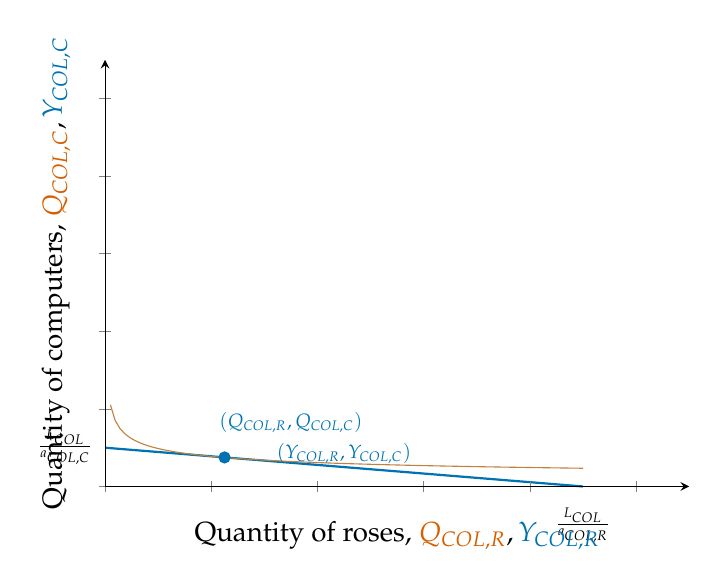
\begin{tikzpicture}
\pgfmathsetmacro{\aC}{900}       % unit labor requirement for computers
\pgfmathsetmacro{\aR}{1}         % unit labor requirement for roses
\pgfmathsetmacro{\alpha}{0.75}    % preference for computers
\pgfmathsetmacro{\Lendow}{9}    % labor endowment

% Compute equilibrium quantities
\pgfmathsetmacro{\Qc}{(\alpha*\Lendow)/\aC}
\pgfmathsetmacro{\Qr}{((1 - \alpha)*\Lendow)/\aR}

% Compute utility level
\pgfmathsetmacro{\U}{(\Qc^(\alpha))*(\Qr^(1 - \alpha))}

% Compute prefactor for indifference curve: Qc = A * Qr^(- (1 - alpha)/alpha)
\pgfmathsetmacro{\expo}{(1 - \alpha)/\alpha}
\pgfmathsetmacro{\A}{\U^(1/\alpha)}

\centering
\begin{axis}[
    ylabel={Quantity of computers, $\textcolor{red}{Q_{COL,C}}, \textcolor{blue}{Y_{COL,C}}$},
    xlabel={Quantity of roses, $\textcolor{red}{Q_{COL,R}}, \textcolor{blue}{Y_{COL,R}}$},
    ymin=0, ymax=0.11,
    xmin=0, xmax=11,
    yticklabel=\empty,
    xticklabel=\empty,
    axis lines=left,
    enlargelimits=false,
    clip=false,
    axis on top,
    scaled x ticks=false,
    width=9cm, height=7cm,
    title style={font=\bfseries}
]

% PPF: Q_C = (L/a_C) - (a_R/a_C) * Q_R
\addplot[thick, blue, domain=0:9] {\Lendow/\aC - (\aR/\aC)*x};

% Indifference curve through optimal bundle
\addplot[brown, domain=0.1:9, samples=100] {\A * x^(-\expo)};

% Labels

%\node at (axis cs:3.5,0.03) {\Large $\mathcal{Y}_{US}$};
\node at (axis cs:\Lendow/\aR,-.01) {\scriptsize $\frac{L_{COL}}{a_{COL,R}}$};
\node at (axis cs:-.75,\Lendow/\aC) {\scriptsize $\frac{L_{COL}}{a_{COL,C}}$};


% Equilibrium point
\addplot[only marks, mark=*, color=blue, mark size=2pt] coordinates {(\Qr, \Qc)};
\node at (axis cs:\Qr + 1.25,\Qc + 0.009) {\scriptsize $\textcolor{blue}{(Q_{COL,R},Q_{COL,C})}$};
\node at (axis cs:\Qr + 2.25,\Qc + 0.001) {\scriptsize $\textcolor{blue}{(Y_{COL,R},Y_{COL,C})}$};


\end{axis}

\end{tikzpicture}
}

\end{subfigure}

\caption{Autarky equilibrium}\label{fig: autarky-num}

\end{figure}

\end{frame}

\begin{frame}{Absolute and Comparative Advantage}

\begin{wideitemize}
    \item We say Colombia has an \textcolor{blue}{absolute advantage} in the production of good $p$ if $a_{COL,p} < a_{US,p}$

    \item English: absolute advantage in production = uses less labor to produce one unit \\
    \qquad \textcolor{gray}{(i.e., it is more productive)}

    \item \textcolor{blue}{Opportunity cost}: cost of producing a good, measured in foregone output of all others.

    \item \blue{Comparative advantage}: An economy has a comparative advantage in producing a good if its opportunity cost of the good is lower than in the rest of the world.

\end{wideitemize}

\end{frame}


\begin{frame}{Absolute and Comparative Advantage}

\begin{wideitemize}

    \item We say Colombia has an \textcolor{blue}{comparative advantage} in the production of roses, since:
    
    \begin{equation*}
        1/900 = a_{COL,R}/a_{COL,C} < a_{US,R}/a_{US,C} = 1/100
    \end{equation*}

    \item We say the US has an \textcolor{blue}{comparative advantage} in the production of computers, since:
    
    \begin{equation*}
        900 = a_{COL,C}/a_{COL,R
        } > a_{US,C}/a_{US,R} = 100
    \end{equation*}

\end{wideitemize}

\end{frame}

\begin{frame}{Global Supply and Demand}

\begin{figure}[htpd!]
\centering
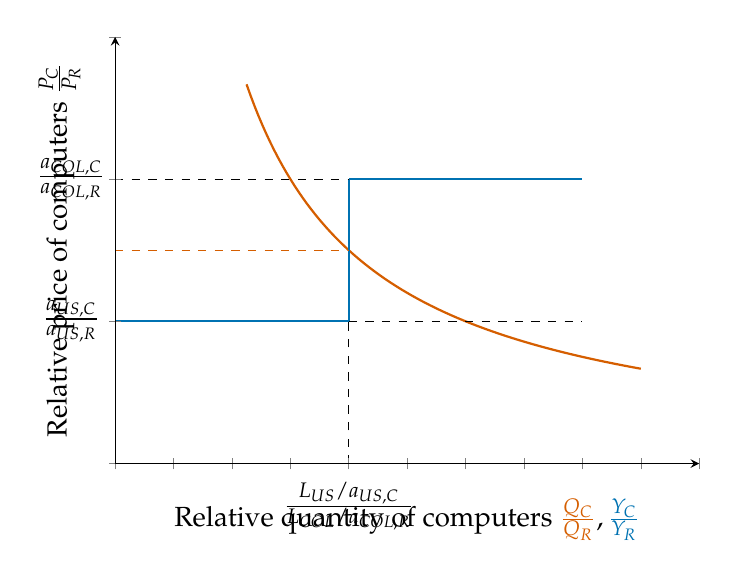
\begin{tikzpicture}
\begin{axis}[
    ylabel={Relative price of computers $\frac{P_C}{P_R}$},
    xlabel={Relative quantity of computers $\textcolor{red}{\frac{Q_{C}}{Q_{R}} } , \textcolor{blue}{\frac{Y_{C}}{Y_{R}} }$},
    ymin=0, ymax=3,
    xmin=0, xmax=2,
    yticklabel=\empty,
    xticklabel=\empty,
    axis lines=left,
    enlargelimits=false,
    clip=false,
    axis on top,
    scaled x ticks=false,
    width=9cm, height=7cm,
    title style={font=\bfseries}]

% Relative Demand RD
\addplot[
    red, thick,
    domain=0.45:1.8,
    samples=100
] {1.2/(x)};
%\node[red] at (axis cs:1.4,1.25) {\small $RD$};

% Relative Supply RS
\addplot[thick, blue] coordinates {(0,1) (0.8,1.0)};
\addplot[thick, blue] coordinates {(0.8,1.0) (0.8,2.0)};
\addplot[thick, blue] coordinates {(0.8,2.0) (1.6,2.0)};
%\node at (axis cs:1.65,2.7) {\small $RS$};

% Dashed lines for autarky prices
\addplot[dashed] coordinates {(0,2.0) (0.8,2.0)};
\node at (axis cs:-0.15,2) {$\frac{a_{COL,C}}{a_{COL,R}}$};

\addplot[dashed] coordinates {(0.8,1.0) (1.6,1.0)};
\node at (axis cs:-0.15,1) {$\frac{a_{US,C}}{a_{US,R}}$};

\addplot[dashed, red] coordinates {(0,1.5) (0.8,1.5)};

% Vertical dashed lines for quantities
\addplot[dashed] coordinates {(0.8,0) (0.8,1.0)};
\node at (axis cs:0.8,-0.3) {$\frac{L_{US}/a_{US,C}}{L_{COL}/a_{COL,R}}$};

\end{axis}
\end{tikzpicture}
\caption{Relative Supply and Demand of Computers as a Function of Relative Prices}
\end{figure}

\end{frame}


\begin{frame}{Production Possibilities Frontier + Trade Prices}
\begin{center}

\begin{figure}[htbp]

% California
\begin{subfigure}{}
\resizebox{0.48\linewidth}{!}{%
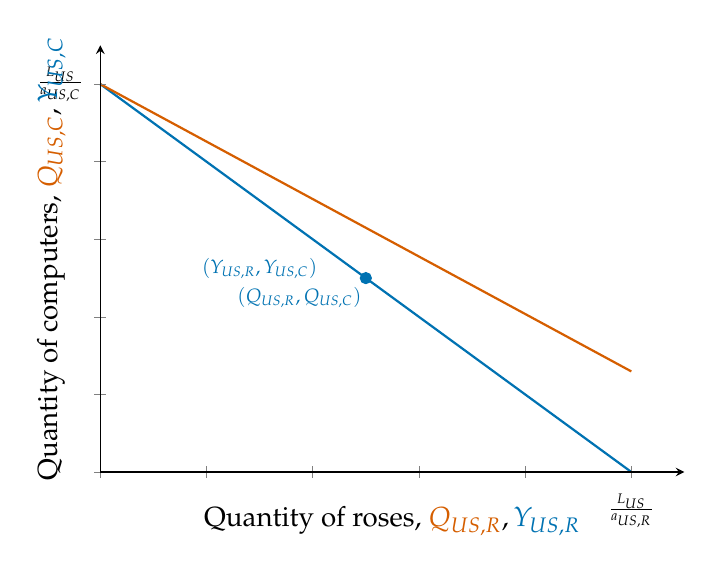
\begin{tikzpicture}
\pgfmathsetmacro{\aC}{100}       % unit labor requirement for computers
\pgfmathsetmacro{\aR}{1}         % unit labor requirement for roses
\pgfmathsetmacro{\alpha}{0.5}    % preference for computers
\pgfmathsetmacro{\Lendow}{10}    % labor endowment

% Compute equilibrium quantities
\pgfmathsetmacro{\Qc}{(\alpha*\Lendow)/\aC}
\pgfmathsetmacro{\Qr}{((1 - \alpha)*\Lendow)/\aR}

% Compute utility level
\pgfmathsetmacro{\U}{(\Qc^(\alpha))*(\Qr^(1 - \alpha))}

% Compute prefactor for indifference curve: Qc = A * Qr^(- (1 - alpha)/alpha)
\pgfmathsetmacro{\expo}{(1 - \alpha)/\alpha}
\pgfmathsetmacro{\A}{\U^(1/\alpha)}

\centering
\begin{axis}[
    ylabel={Quantity of computers, $\textcolor{red}{Q_{US,C}}, \textcolor{blue}{Y_{US,C}}$},
    xlabel={Quantity of roses, $\textcolor{red}{Q_{US,R}}, \textcolor{blue}{Y_{US,R}}$},
    ymin=0, ymax=0.11,
    xmin=0, xmax=11,
    yticklabel=\empty,
    xticklabel=\empty,
    axis lines=left,
    enlargelimits=false,
    clip=false,
    axis on top,
    scaled x ticks=false,
    width=9cm, height=7cm,
    title style={font=\bfseries}
]

% PPF: Q_C = (L/a_C) - (a_R/a_C) * Q_R
\addplot[thick, blue, domain=0:10] {\Lendow/\aC - (\aR/\aC)*x};

\addplot[thick, red, domain=0:10] {\Lendow/\aC - (1/135)*x};


% Indifference curve through optimal bundle
%\addplot[red, domain=0.1:9, samples=100] {\A * x^(-\expo)};

% Labels

%\node at (axis cs:3.5,0.03) {\Large $\mathcal{Y}_{US}$};
\node at (axis cs:\Lendow/\aR,-.01) {\scriptsize $\frac{L_{US}}{a_{US,R}}$};
\node at (axis cs:-.75,\Lendow/\aC) {\scriptsize $\frac{L_{US}}{a_{US,C}}$};


% Equilibrium point
\addplot[only marks, mark=*, color=blue, mark size=2pt] coordinates {(\Qr, \Qc)};
\node at (axis cs:\Qr - 1.25,\Qc - 0.005) {\scriptsize $\textcolor{blue}{(Q_{US,R},Q_{US,C})}$};
\node at (axis cs:\Qr - 2,\Qc + 0.0025) {\scriptsize $\textcolor{blue}{(Y_{US,R},Y_{US,C})}$};

\end{axis}

\end{tikzpicture}
}
\end{subfigure}
%
% Colombia
\begin{subfigure}{}
\resizebox{0.48\linewidth}{!}{%
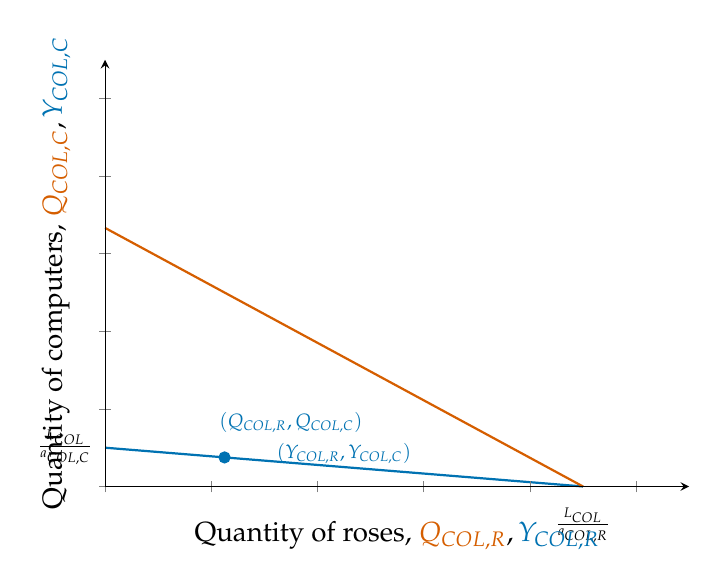
\begin{tikzpicture}
\pgfmathsetmacro{\aC}{900}       % unit labor requirement for computers
\pgfmathsetmacro{\aR}{1}         % unit labor requirement for roses
\pgfmathsetmacro{\alpha}{0.75}    % preference for computers
\pgfmathsetmacro{\Lendow}{9}    % labor endowment

% Compute equilibrium quantities
\pgfmathsetmacro{\Qc}{(\alpha*\Lendow)/\aC}
\pgfmathsetmacro{\Qr}{((1 - \alpha)*\Lendow)/\aR}

% Compute utility level
\pgfmathsetmacro{\U}{(\Qc^(\alpha))*(\Qr^(1 - \alpha))}

% Compute prefactor for indifference curve: Qc = A * Qr^(- (1 - alpha)/alpha)
\pgfmathsetmacro{\expo}{(1 - \alpha)/\alpha}
\pgfmathsetmacro{\A}{\U^(1/\alpha)}

\centering
\begin{axis}[
    ylabel={Quantity of computers, $\textcolor{red}{Q_{COL,C}}, \textcolor{blue}{Y_{COL,C}}$},
    xlabel={Quantity of roses, $\textcolor{red}{Q_{COL,R}}, \textcolor{blue}{Y_{COL,R}}$},
    ymin=0, ymax=0.11,
    xmin=0, xmax=11,
    yticklabel=\empty,
    xticklabel=\empty,
    axis lines=left,
    enlargelimits=false,
    clip=false,
    axis on top,
    scaled x ticks=false,
    width=9cm, height=7cm,
    title style={font=\bfseries}
]

% PPF: Q_C = (L/a_C) - (a_R/a_C) * Q_R
\addplot[thick, blue, domain=0:9] {\Lendow/\aC - (\aR/\aC)*x};

\addplot[thick, red, domain=0:9] {1/15 - (1/135)*x};


% Indifference curve through optimal bundle
%\addplot[red, domain=0.1:9, samples=100] {\A * x^(-\expo)};

% Labels

%\node at (axis cs:3.5,0.03) {\Large $\mathcal{Y}_{US}$};
\node at (axis cs:\Lendow/\aR,-.01) {\scriptsize $\frac{L_{COL}}{a_{COL,R}}$};
\node at (axis cs:-.75,\Lendow/\aC) {\scriptsize $\frac{L_{COL}}{a_{COL,C}}$};


% Equilibrium point
\addplot[only marks, mark=*, color=blue, mark size=2pt] coordinates {(\Qr, \Qc)};
\node at (axis cs:\Qr + 1.25,\Qc + 0.009) {\scriptsize $\textcolor{blue}{(Q_{COL,R},Q_{COL,C})}$};
\node at (axis cs:\Qr + 2.25,\Qc + 0.001) {\scriptsize $\textcolor{blue}{(Y_{COL,R},Y_{COL,C})}$};

\end{axis}

\end{tikzpicture}
}

\end{subfigure}

\caption{Autarky Equilibrium + Trade Prices}
\end{figure}
\end{center}
\end{frame}


\begin{frame}{Production Possibilities Frontier + Trade Prices + Specialization}
\begin{center}

\begin{figure}[htbp]

% California
\begin{subfigure}{}
\resizebox{0.48\linewidth}{!}{%
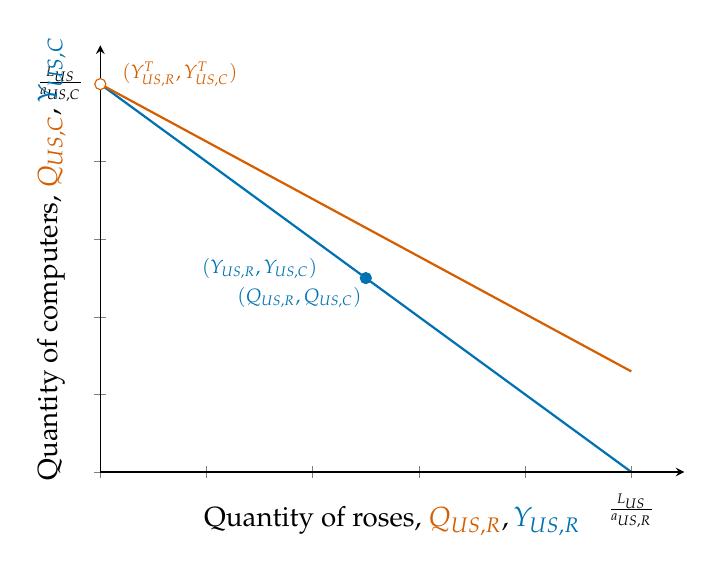
\begin{tikzpicture}
\pgfmathsetmacro{\aC}{100}       % unit labor requirement for computers
\pgfmathsetmacro{\aR}{1}         % unit labor requirement for roses
\pgfmathsetmacro{\alpha}{0.5}    % preference for computers
\pgfmathsetmacro{\Lendow}{10}    % labor endowment

% Compute equilibrium quantities
\pgfmathsetmacro{\Qc}{(\alpha*\Lendow)/\aC}
\pgfmathsetmacro{\Qr}{((1 - \alpha)*\Lendow)/\aR}

% Compute utility level
\pgfmathsetmacro{\U}{(\Qc^(\alpha))*(\Qr^(1 - \alpha))}

% Compute prefactor for indifference curve: Qc = A * Qr^(- (1 - alpha)/alpha)
\pgfmathsetmacro{\expo}{(1 - \alpha)/\alpha}
\pgfmathsetmacro{\A}{\U^(1/\alpha)}

\centering
\begin{axis}[
    ylabel={Quantity of computers, $\textcolor{red}{Q_{US,C}}, \textcolor{blue}{Y_{US,C}}$},
    xlabel={Quantity of roses, $\textcolor{red}{Q_{US,R}}, \textcolor{blue}{Y_{US,R}}$},
    ymin=0, ymax=0.11,
    xmin=0, xmax=11,
    yticklabel=\empty,
    xticklabel=\empty,
    axis lines=left,
    enlargelimits=false,
    clip=false,
    axis on top,
    scaled x ticks=false,
    width=9cm, height=7cm,
    title style={font=\bfseries}
]

% PPF: Q_C = (L/a_C) - (a_R/a_C) * Q_R
\addplot[thick, blue, domain=0:10] {\Lendow/\aC - (\aR/\aC)*x};

\addplot[thick, red, domain=0:10] {\Lendow/\aC - (1/135)*x};


% Indifference curve through optimal bundle
%\addplot[red, domain=0.1:9, samples=100] {\A * x^(-\expo)};

% Labels

%\node at (axis cs:3.5,0.03) {\Large $\mathcal{Y}_{US}$};
\node at (axis cs:\Lendow/\aR,-.01) {\scriptsize $\frac{L_{US}}{a_{US,R}}$};
\node at (axis cs:-.75,\Lendow/\aC) {\scriptsize $\frac{L_{US}}{a_{US,C}}$};


% Equilibrium point
\addplot[only marks, mark=*, color=blue, mark size=2pt] coordinates {(\Qr, \Qc)};
\node at (axis cs:\Qr - 1.25,\Qc - 0.005) {\scriptsize $\textcolor{blue}{(Q_{US,R},Q_{US,C})}$};
\node at (axis cs:\Qr - 2,\Qc + 0.0025) {\scriptsize $\textcolor{blue}{(Y_{US,R},Y_{US,C})}$};

\addplot[only marks, mark=*, mark options={fill=white, draw=red}, mark size=2pt] coordinates {(0, \Lendow/\aC)};
\node at (axis cs:0 + 1.5,\Lendow/\aC + 0.0025) {\scriptsize $\textcolor{red}{(Y^T_{US,R},Y^T_{US,C})}$};

\end{axis}

\end{tikzpicture}
}
\end{subfigure}
%
% Colombia
\begin{subfigure}{}
\resizebox{0.48\linewidth}{!}{%
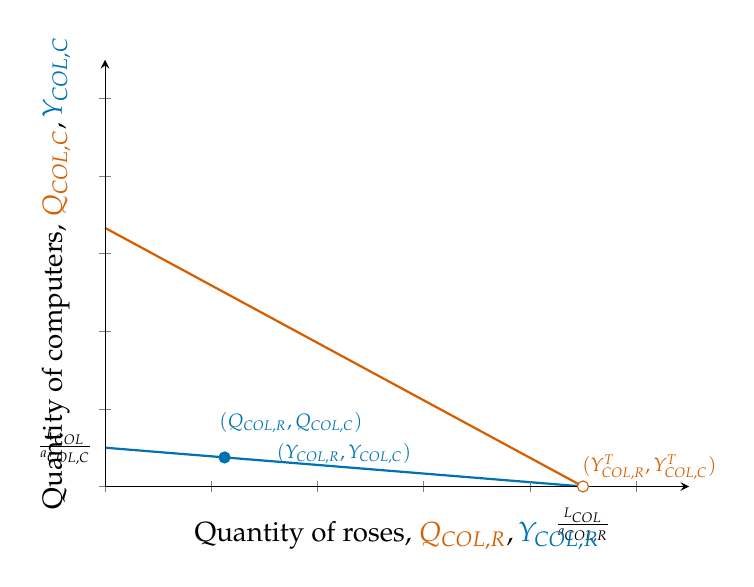
\begin{tikzpicture}
\pgfmathsetmacro{\aC}{900}       % unit labor requirement for computers
\pgfmathsetmacro{\aR}{1}         % unit labor requirement for roses
\pgfmathsetmacro{\alpha}{0.75}    % preference for computers
\pgfmathsetmacro{\Lendow}{9}    % labor endowment

% Compute equilibrium quantities
\pgfmathsetmacro{\Qc}{(\alpha*\Lendow)/\aC}
\pgfmathsetmacro{\Qr}{((1 - \alpha)*\Lendow)/\aR}

% Compute utility level
\pgfmathsetmacro{\U}{(\Qc^(\alpha))*(\Qr^(1 - \alpha))}

% Compute prefactor for indifference curve: Qc = A * Qr^(- (1 - alpha)/alpha)
\pgfmathsetmacro{\expo}{(1 - \alpha)/\alpha}
\pgfmathsetmacro{\A}{\U^(1/\alpha)}

\centering
\begin{axis}[
    ylabel={Quantity of computers, $\textcolor{red}{Q_{COL,C}}, \textcolor{blue}{Y_{COL,C}}$},
    xlabel={Quantity of roses, $\textcolor{red}{Q_{COL,R}}, \textcolor{blue}{Y_{COL,R}}$},
    ymin=0, ymax=0.11,
    xmin=0, xmax=11,
    yticklabel=\empty,
    xticklabel=\empty,
    axis lines=left,
    enlargelimits=false,
    clip=false,
    axis on top,
    scaled x ticks=false,
    width=9cm, height=7cm,
    title style={font=\bfseries}
]

% PPF: Q_C = (L/a_C) - (a_R/a_C) * Q_R
\addplot[thick, blue, domain=0:9] {\Lendow/\aC - (\aR/\aC)*x};

\addplot[thick, red, domain=0:9] {1/15 - (1/135)*x};


% Indifference curve through optimal bundle
%\addplot[red, domain=0.1:9, samples=100] {\A * x^(-\expo)};

% Labels

%\node at (axis cs:3.5,0.03) {\Large $\mathcal{Y}_{US}$};
\node at (axis cs:\Lendow/\aR,-.01) {\scriptsize $\frac{L_{COL}}{a_{COL,R}}$};
\node at (axis cs:-.75,\Lendow/\aC) {\scriptsize $\frac{L_{COL}}{a_{COL,C}}$};


% Equilibrium point
\addplot[only marks, mark=*, color=blue, mark size=2pt] coordinates {(\Qr, \Qc)};
\node at (axis cs:\Qr + 1.25,\Qc + 0.009) {\scriptsize $\textcolor{blue}{(Q_{COL,R},Q_{COL,C})}$};
\node at (axis cs:\Qr + 2.25,\Qc + 0.001) {\scriptsize $\textcolor{blue}{(Y_{COL,R},Y_{COL,C})}$};

\addplot[only marks, mark=*, mark options={fill=white, draw=red}, mark size=2pt] coordinates {(\Lendow/\aR, 0)};
\node at (axis cs:\Lendow/\aR + 1.25,0 + 0.005) {\scriptsize $\textcolor{red}{(Y^T_{COL,R},Y^T_{COL,C})}$};

\end{axis}

\end{tikzpicture}
}

\end{subfigure}

\caption{Production under Free Trade induces Specialization}

\end{figure}
\end{center}
\end{frame}

\begin{frame}{Trade Equilibrium}
\begin{center}


\begin{figure}[htbp]

% California
\begin{subfigure}{}
\resizebox{0.48\linewidth}{!}{%
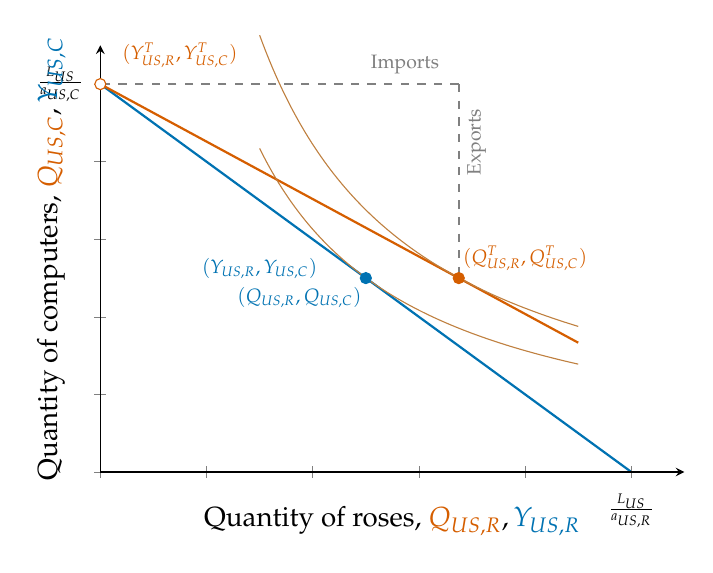
\begin{tikzpicture}
\pgfmathsetmacro{\aC}{100}       % unit labor requirement for computers
\pgfmathsetmacro{\aR}{1}         % unit labor requirement for roses
\pgfmathsetmacro{\alpha}{0.5}    % preference for computers
\pgfmathsetmacro{\Lendow}{10}    % labor endowment
\pgfmathsetmacro{\p}{135}    % trade price

% Compute equilibrium quantities
\pgfmathsetmacro{\Qc}{(\alpha*\Lendow)/\aC}
\pgfmathsetmacro{\Qr}{((1 - \alpha)*\Lendow)/\aR}
\pgfmathsetmacro{\QcT}{(\alpha*\Lendow)/\aC}
\pgfmathsetmacro{\QrT}{((1 - \alpha)*\p*\Lendow)/\aC}

% Compute utility level
\pgfmathsetmacro{\U}{(\Qc^(\alpha))*(\Qr^(1 - \alpha))}
\pgfmathsetmacro{\UT}{(\QcT^(\alpha))*(\QrT^(1 - \alpha))}

% Compute prefactor for indifference curve: Qc = A * Qr^(- (1 - alpha)/alpha)
\pgfmathsetmacro{\expo}{(1 - \alpha)/\alpha}
\pgfmathsetmacro{\A}{\U^(1/\alpha)}
\pgfmathsetmacro{\AT}{\UT^(1/\alpha)}

\centering
\begin{axis}[
    ylabel={Quantity of computers, $\textcolor{red}{Q_{US,C}}, \textcolor{blue}{Y_{US,C}}$},
    xlabel={Quantity of roses, $\textcolor{red}{Q_{US,R}}, \textcolor{blue}{Y_{US,R}}$},
    ymin=0, ymax=\Lendow/\aC * 1.1,
    xmin=0, xmax=\Lendow/\aR * 1.1,
    yticklabel=\empty,
    xticklabel=\empty,
    axis lines=left,
    enlargelimits=false,
    clip=false,
    axis on top,
    scaled x ticks=false,
    width=9cm, height=7cm,
    title style={font=\bfseries}
]

% PPF: Q_C = (L/a_C) - (a_R/a_C) * Q_R
\addplot[thick, blue, domain=0:10] {\Lendow/\aC - (\aR/\aC)*x};
\addplot[thick, red, domain=0:9] {\Lendow/\aC  - (1/\p)*x};

% Indifference curve through optimal bundle
\addplot[brown, domain=3:9, samples=100] {\A * x^(-\expo)};
\addplot[brown, domain=3:9, samples=100] {\AT * x^(-\expo)};

% Labels

%\node at (axis cs:3.5,0.03) {\Large $\mathcal{Y}_{US}$};
\node at (axis cs:\Lendow/\aR,-.01) {\scriptsize $\frac{L_{US}}{a_{US,R}}$};
\node at (axis cs:-.75,\Lendow/\aC) {\scriptsize $\frac{L_{US}}{a_{US,C}}$};

% Equilibrium point
\addplot[only marks, mark=*, color=blue, mark size=2pt] coordinates {(\Qr, \Qc)};
\node at (axis cs:\Qr - 1.25,\Qc - 0.005) {\scriptsize $\textcolor{blue}{(Q_{US,R},Q_{US,C})}$};
\node at (axis cs:\Qr - 2,\Qc + 0.0025) {\scriptsize $\textcolor{blue}{(Y_{US,R},Y_{US,C})}$};

\addplot[only marks, mark=*, color=red, mark size=2pt] coordinates {(\QrT, \QcT)};
\node at (axis cs:\QrT + 1.25,\QcT + 0.005) {\scriptsize $\textcolor{red}{(Q^T_{US,R},Q^T_{US,C})}$};

\addplot[only marks, mark=*, mark options={fill=white, draw=red}, mark size=2pt] coordinates {(0, \Lendow/\aC)};
\node at (axis cs:0 + 1.5,\Lendow/\aC + 0.0075) {\scriptsize $\textcolor{red}{(Y^T_{US,R},Y^T_{US,C})}$};

% Arrows for exports (horizontal)
\draw[-, dashed, thick, gray] 
    (axis cs:\QrT,\Lendow/\aC) -- 
    (axis cs:0,\Lendow/\aC);
\node[gray] at (axis cs:\QrT*0.85,\Lendow/\aC*1.05) {\scriptsize Imports};

% Arrows for imports (vertical)
\draw[-, dashed, thick, gray] 
    (axis cs:\QrT,\Lendow/\aC) -- 
    (axis cs:\QrT, \QcT);
\node[gray, rotate=90] at (axis cs:\QrT*1.05,\Lendow/\aC*0.85) {\scriptsize Exports};



\end{axis}

\end{tikzpicture}
}
\end{subfigure}
%
% Colombia
\begin{subfigure}{}
\resizebox{0.48\linewidth}{!}{%

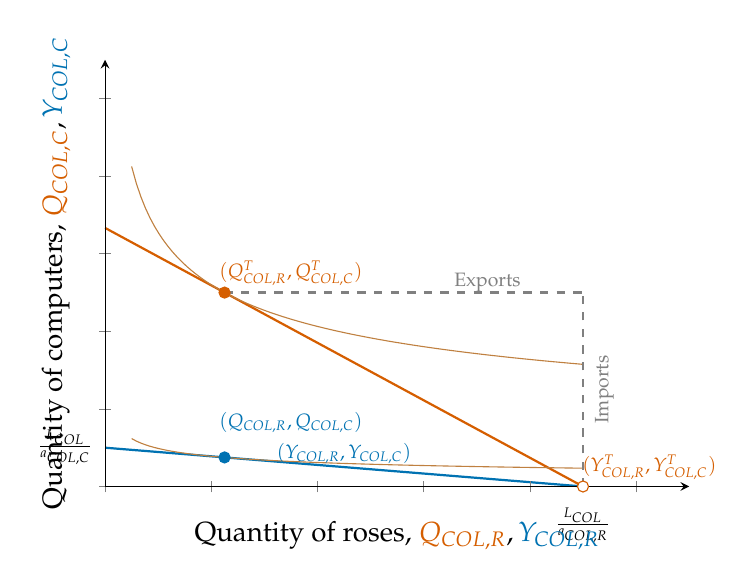
\begin{tikzpicture}
\pgfmathsetmacro{\aC}{900}       % unit labor requirement for computers
\pgfmathsetmacro{\aR}{1}         % unit labor requirement for roses
\pgfmathsetmacro{\alpha}{0.75}    % preference for computers
\pgfmathsetmacro{\Lendow}{9}    % labor endowment
\pgfmathsetmacro{\p}{135}    % trade price


% Compute equilibrium quantities
\pgfmathsetmacro{\Qc}{(\alpha*\Lendow)/\aC}
\pgfmathsetmacro{\Qr}{((1 - \alpha)*\Lendow)/\aR}
\pgfmathsetmacro{\QcT}{(\alpha*\Lendow)/(\aR*\p)}
\pgfmathsetmacro{\QrT}{((1 - \alpha)*\Lendow)/\aR}

% Compute prefactor for indifference curve: Qc = A * Qr^(- (1 - alpha)/alpha)
\pgfmathsetmacro{\expo}{(1 - \alpha)/\alpha}
\pgfmathsetmacro{\A}{\Qc * \Qr^((1 - \alpha)/\alpha))}
\pgfmathsetmacro{\AT}{\QcT * \QrT^((1 - \alpha)/\alpha))}

\centering
\begin{axis}[
    ylabel={Quantity of computers, $\textcolor{red}{Q_{COL,C}}, \textcolor{blue}{Y_{COL,C}}$},
    xlabel={Quantity of roses, $\textcolor{red}{Q_{COL,R}}, \textcolor{blue}{Y_{COL,R}}$},
    ymin=0, ymax=0.11,
    xmin=0, xmax=11,
    yticklabel=\empty,
    xticklabel=\empty,
    axis lines=left,
    enlargelimits=false,
    clip=false,
    axis on top,
    scaled x ticks=false,
    width=9cm, height=7cm,
    title style={font=\bfseries}
]

% PPF: Q_C = (L/a_C) - (a_R/a_C) * Q_R
\addplot[thick, blue, domain=0:9] {\Lendow/\aC - (\aR/\aC)*x};
\addplot[thick, red, domain=0:9] {\Lendow/\aR * 1/ \p - (1/\p)*x};


% Indifference curve through optimal bundle
\addplot[brown, domain=0.5:9, samples=100] {\A * x^(-\expo)};
\addplot[brown, domain=0.5:9, samples=100] {\AT * x^(-\expo)};

% Labels

%\node at (axis cs:3.5,0.03) {\Large $\mathcal{Y}_{US}$};
\node at (axis cs:\Lendow/\aR,-.01) {\scriptsize $\frac{L_{COL}}{a_{COL,R}}$};
\node at (axis cs:-.75,\Lendow/\aC) {\scriptsize $\frac{L_{COL}}{a_{COL,C}}$};


% Equilibrium point
\addplot[only marks, mark=*, color=blue, mark size=2pt] coordinates {(\Qr, \Qc)};
\node at (axis cs:\Qr + 1.25,\Qc + 0.009) {\scriptsize $\textcolor{blue}{(Q_{COL,R},Q_{COL,C})}$};
\node at (axis cs:\Qr + 2.25,\Qc + 0.001) {\scriptsize $\textcolor{blue}{(Y_{COL,R},Y_{COL,C})}$};


\addplot[only marks, mark=*, color=red, mark size=2pt] coordinates {(\QrT, \QcT)};
\node at (axis cs:\QrT + 1.25,\QcT + 0.005) {\scriptsize $\textcolor{red}{(Q^T_{COL,R},Q^T_{COL,C})}$};

\addplot[only marks, mark=*, mark options={fill=white, draw=red}, mark size=2pt] coordinates {(\Lendow/\aR, 0)};
\node at (axis cs:\Lendow/\aR + 1.25,0 + 0.005) {\scriptsize $\textcolor{red}{(Y^T_{COL,R},Y^T_{COL,C})}$};

% Arrows for exports (horizontal)
\draw[-, dashed, thick, gray] 
    (axis cs:\QrT,\QcT) -- 
    (axis cs:\Lendow/\aR,\QcT);
\node[gray] at (axis cs:{ \Lendow/\aR *0.8}, \QcT*1.05) {\scriptsize Exports};

% Arrows for imports (vertical)
\draw[-, dashed, thick, gray] 
    (axis cs:{\Lendow/\aR},0) -- 
    (axis cs:{\Lendow/\aR}, \QcT);
\node[gray, rotate=90] at (axis cs:{\Lendow/\aR + 0.4}, {\QcT/2}) {\scriptsize Imports};

\end{axis}

\end{tikzpicture}
}

\end{subfigure}

\caption{Specialization + Trade Equilibrium}

\end{figure}

\end{center}

\end{frame}

\section{Ricardo with Multiple Goods}

\begin{frame}
\addtocounter{framenumber}{-1}

\centering

\Huge{\blue{Ricardian Model with Multiple Goods}}
    
\end{frame}

\begin{frame}{Ricardian Model with Multiple Goods: Preliminaries}
\begin{wideitemize}
        \item 2 countries $i \in \{ H, F\}$
        \item Many goods indexed (labeled) $g \in [0,1]$
        \item One factor of production: labor $L_i$ mobile between sectors
        \item In country $i$, to produce one unit of good $g$, firms use $a_{i,g}$ units of labor
        \item Firms (potentially) producing good $g$ maximize $\max_{y_{i,g}} p_{g} y_{i,g} - w_i a_{i,g} y_{i,g}$
        \item Consumers have identical preferences over all goods: $q_{i,g} = \frac{w_iL_i}{P_{i,g}}$
        \item Trade balances (value of exports = value of imports)
        \end{wideitemize}
\end{frame}

\begin{frame}{Perfect Competition, Prices and Unit Costs}
\begin{wideitemize}
        \item In country $i$, firms producing good $g$ maximize profits under perfect competition:
        \begin{equation*}
            \max_{y_{i,g}} \pi_{i,g} = \max_{y_{i,g}} p_{g} y_{i,g} - w_i a_{i,g} y_{i,g} 
        \end{equation*}

        \item Under perfect competition, goods prices reflect unit cost:
        \begin{itemize}
            \item If home makes $g$, its factory-gate price is $P_g = a_{H,g} w_{H}$
            \item If foreign makes $g$, its factory-gate price is $P_g = a_{F,g} w_{F}$
        \end{itemize}
    \item Production only if cheaper to produce domestically than to import goods, i.e.:

    \begin{equation*}
        w_H a_{H,g} \le w_F a_{F,g} \text{ or, equivalently, if } \frac{w_H}{w_F} \le  \frac{a_{F,g}}{a_{H,g}}
    \end{equation*}

    \item \blue{Prices}: price of good $g$ will be the lowest of unit costs at home or abroad:


        \begin{equation*}
            P_{g} = \min\{w_H a_{H,g}, w_F a_{F,g}\}  \qquad \text{ for } g \in [0,1]
        \end{equation*}
        \end{wideitemize}
\end{frame}


\begin{frame}{Where will production be located?}
\begin{wideitemize}
    \item \blue{Assumption}: order goods $g \in [0,1]$ according to the home country's comparative advantage.

     \item \blue{Define}: $A_g \equiv  a_{F,g}/ a_{H,g}$. $\implies$ $A_g$ strictly decreasing in $g$.

     \begin{itemize}
         \item $A_0= \frac{a_{F,0}}{a_{H,0}}$: home is the \blue{most productive}
         \item $A_1= \frac{a_{F,1}}{a_{H,1}}$: home is the \blue{least productive} 
     \end{itemize}

            
        \end{wideitemize}
\end{frame}

\begin{frame}{Relative cost schedule}
    \begin{figure}
        \centering
        \begin{tikzpicture}
        \begin{axis}[
            axis lines=left,
            xmin=0, xmax=1.05,
            ymin=0, ymax=1.05,
            ylabel={$A_g$},
            xtick={0,1},
            ytick={0,1},
            xticklabels={0, 1},
            yticklabels={0, 1},
            tick style={draw=none},
            xticklabel style={anchor=north west, yshift=0pt},
            yticklabel style={anchor=south east, xshift=0pt},
            enlargelimits=false,
            clip=false,
            grid=major,
            width=0.7\textwidth,
            height=0.45\textwidth,
            label style={font=\small},
            tick label style={font=\small},
        ]
        

            % Relative cost schedule
            \addplot[red, thick, domain=0.02:1] {x^(-1/6) - 0.975};
           
            \end{axis}
        \end{tikzpicture}
        \caption{Relative unit labor costs $A_g = a_{F,g} / a_{H,g}$}
        \label{fig:Ap}
    \end{figure}
\end{frame}


\begin{frame}{Equilibrium}
\begin{wideitemize}
    \item<1-> In equilibrium there will be some cut-off good $G$ for which:

    \begin{equation*}
        \frac{w_H}{w_F} = A_G
    \end{equation*}

     \item<2-> Since $A_g$ is decreasing in $g$, then:

     \begin{itemize}
         \item Goods $[0,G]$ will be produced at home (for them, $w_H / w_F \le A_g$)
         \item Goods $(G,1]$ will be produced at abroad (for them, $w_H / w_F > A_g$)
        \end{itemize}

        \item<3-> Recall: trade pattern and specialization depends on Home-to-Foreign wage ratio (gap) $w_H/w_F$ 

    \end{wideitemize}
\end{frame}

\begin{frame}{Specialization}
    \begin{figure}
        \centering
        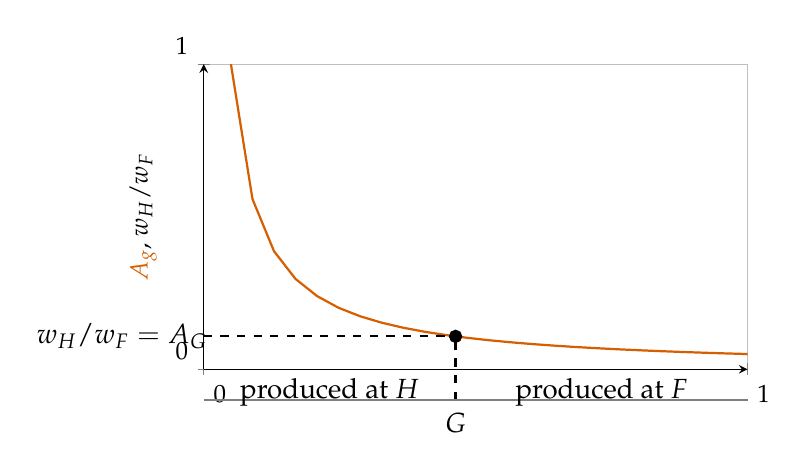
\begin{tikzpicture}
            \begin{axis}[
                axis lines=left,
                xmin=0, xmax=1,
                ymin=0, ymax=1,
                ylabel={\textcolor{red}{$A_g$}, $w_H/w_F$},
                xtick={0,1},
                ytick={0,1},
                xticklabels={0, 1},
                xticklabel style={anchor=north west, yshift=0pt},
                yticklabel style={anchor=south east, xshift=0pt},
                enlargelimits=false,
                clip=false,
                grid=major,
                width=12cm,
                height=8cm,
                every axis plot/.style={thick},
                width=0.7\textwidth,
                height=0.45\textwidth,
                label style={font=\small},
                tick label style={font=\small},
            ]
                       
            \pgfmathsetmacro{\z}{0.05}       
            \pgfmathsetmacro{\c}{0.125}         
            \pgfmathsetmacro{\x}{ (-\z + sqrt(\z^2 + 4*\c*\z)) / (2*\c) }
            \pgfmathsetmacro{\y}{ \z / \x  }         
            \addplot[red, thick, domain=0.05:1] {\z / x}; % A_g
            
            \addplot[dashed] coordinates {(0,\y) (\x,\y)};
            \node at (axis cs:-0.15,\y) {$w_H/w_F=A_G$};
            \addplot[dashed] coordinates {(\x,-.1) (\x,\y)};
            \node at (axis cs:\x,-0.175) {$G$};
            \addplot[gray] coordinates {(0,-0.1) (\x,-0.1)};
            \node at (axis cs:\x/2,-0.075) {produced at $H$};
            \addplot[gray] coordinates {(\x,-0.1) (1,-0.1)};
            \node at (axis cs:( {\x + (1-\x)/2},-0.075) {produced at $F$};
            
            \addplot[only marks, mark=*, color=black, mark size=2pt] coordinates {(\x, \y)};

            \end{axis}
            \end{tikzpicture}
        \caption{Relative unit labor costs $A_g = a_{F,g} / a_{H,g}$}
        \label{fig: Ag}
    \end{figure}

    
\end{frame}

\begin{frame}{Equilibrium determination}
\begin{wideitemize}
    \item Recall:
    \begin{itemize}
        \item Home produces $G$ share of goods
        \item Foreign produces $1-G$ share of goods
        \item Consumers spend the same amount on each good
    \end{itemize}

    \item $\implies$ consumers in each country spend $G$ share of their income on goods from $H$

    \item How to find $G?$ 

    \begin{eqnarray*}
        \underbrace{w_HL_H}_{\text{income}} = \underbrace{G\times w_HL_H + G\times w_FL_F}_{\text{expenditure}} \iff w_HL_H = \frac{G}{1-G}w_FL_F
    \end{eqnarray*}

    \item Or, solving for $w_H / w_F$:

    \begin{equation*}
        \frac{w_H}{w_F} =  \frac{G}{1-G} \frac{L_F}{L_H}
    \end{equation*}
    
    \end{wideitemize}
\end{frame}


\begin{frame}{Equilibrium determination}
    \begin{figure}
        \centering
        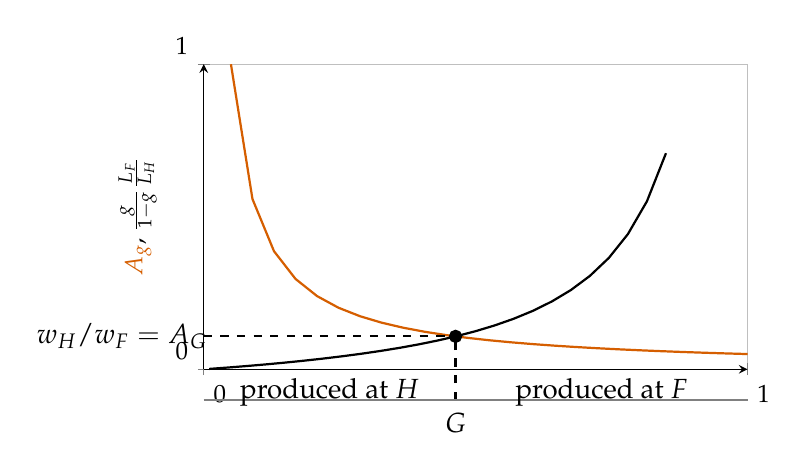
\begin{tikzpicture}
            \begin{axis}[
                axis lines=left,
                xmin=0, xmax=1,
                ymin=0, ymax=1,
                ylabel={\textcolor{red}{$A_g$}, $\frac{g}{1-g} \frac{L_F}{L_H}$},
                xtick={0,1},
                ytick={0,1},
                xticklabels={0, 1},
                xticklabel style={anchor=north west, yshift=0pt},
                yticklabel style={anchor=south east, xshift=0pt},
                enlargelimits=false,
                clip=false,
                grid=major,
                width=12cm,
                height=8cm,
                every axis plot/.style={thick},
                width=0.7\textwidth,
                height=0.45\textwidth,
                label style={font=\small},
                tick label style={font=\small},
            ]
                       
            \pgfmathsetmacro{\z}{0.05}       
            \pgfmathsetmacro{\c}{0.125}         
            \pgfmathsetmacro{\x}{ (-\z + sqrt(\z^2 + 4*\c*\z)) / (2*\c) }
            \pgfmathsetmacro{\y}{ \z / \x  }         
            \addplot[red, thick, domain=0.05:1] {\z / x}; % A_g
            \addplot[black, thick, domain=0.01:0.85] {x / (1 - x) * \c}; % omega(g)
            
            \addplot[dashed] coordinates {(0,\y) (\x,\y)};
            \node at (axis cs:-0.15,\y) {$w_H/w_F=A_G$};
            \addplot[dashed] coordinates {(\x,-.1) (\x,\y)};
            \node at (axis cs:\x,-0.175) {$G$};
            \addplot[gray] coordinates {(0,-0.1) (\x,-0.1)};
            \node at (axis cs:\x/2,-0.075) {produced at $H$};
            \addplot[gray] coordinates {(\x,-0.1) (1,-0.1)};
            \node at (axis cs:( {\x + (1-\x)/2},-0.075) {produced at $F$};
            
            \addplot[only marks, mark=*, color=black, mark size=2pt] coordinates {(\x, \y)};

            \end{axis}
            \end{tikzpicture}
        \caption{Relative unit labor costs $A_g = a_{F,g} / a_{H,g}$}
        \label{fig: Ag}
    \end{figure}
    \end{frame}

\section{Production Model}

\begin{frame}
\addtocounter{framenumber}{-1}

\centering

\Huge{\blue{Production Model}}
    
\end{frame}

\begin{frame}{Production Model: Preliminaries}
\begin{wideitemize}
        \item Single country, single product
        \item Two factors of production: capital $K$ and labor $L$ 
        \item Production represented by a production function $F(K,L)$
        \item Firms maximize profits = revenue - costs
        \item Supply of capital and labor inelastic  
        \item Prices adjust to make sure supply = demand
    \end{wideitemize}
\end{frame}



\begin{frame}{The Production Function}

\begin{wideitemize}
\item We are interested in modeling the production of some ``output'' good
\item We will take a “factor‐based” representation of the production function:

\begin{equation*}
\underbrace{Y}_{\substack{\text{output}}} = F(\underbrace{\bar{Z}}_{\substack{\text{technology}\\\text{institutions}\\\text{ideas}}}, \underbrace{K}_{\text{capital}} , \underbrace{L}_{\text{labor}})
\end{equation*}

\item $F(\bar{Z}, K, L)$ is your production function. If $F(\cdot, \cdot, \cdot)$ is Cobb-Douglas, then:

\begin{equation*}
    Y = \bar{Z} \cdot K^{\beta} L^{1-\beta}, \qquad 0 \le \beta \le 1  
\end{equation*}

\end{wideitemize}

\end{frame}


\begin{frame}{Production Function}
  \Large{\textcolor{blue}{Diminishing Marginal Product}: Extra output produced by increasing one factor
while keeping all the other fixed is decreasing in the one increasing factor.} \\
\onslide<2->{
  \vspace{20pt}
  \normalsize With Cobb-Douglas Technology, the Marginal Product of Labor and Capital are:
  \vspace{20pt}
  \begin{columns}[T] % align columns
\begin{column}{.5\textwidth}
\begin{equation*}
  MPL \equiv \frac{\partial Y}{\partial L} = \underbrace{(1-\beta) \bar{Z} \left( \frac{K}{L} \right)^{\beta}}_{\text{decreasing in } L}
\end{equation*}
\end{column}%
\hfill%
\begin{column}{.5\textwidth}
\begin{equation*}
  MPK \equiv \frac{\partial Y}{\partial K} = \underbrace{\beta \bar{Z} \left( \frac{L}{K} \right)^{1-\beta}}_{\text{decreasing in } K}
\end{equation*}

\end{column}%
\end{columns}
}
\end{frame}


\begin{frame}{Example: Capital}

\begin{columns}[T] % align columns
\begin{column}{.6\textwidth}
  \makebox[\linewidth][c]{
    \resizebox{\linewidth}{!}{
  
    \begin{tikzpicture}
    \pgfmathsetmacro{\alpha}{2/3}    % preference for computers
    \pgfmathsetmacro{\K}{1}    % labor endowment
    \pgfmathsetmacro{\A}{1}    % labor endowment
    
    \centering
    \begin{axis}[
        ylabel={$Y = Z \times K^{1/3} L^{2/3}$ },
        xlabel={Used capital input: $K$},
        ymin=0, ymax=5,
        xmin=0, xmax=5,
        yticklabel=\empty,
        xticklabel=\empty,
        axis lines=left,
        enlargelimits=false,
        clip=false,
        axis on top,
        scaled x ticks=false,
        width=9cm, height=7cm,
        title style={font=\bfseries}
    ]
    
    % PPF: Q_C = (L/a_C) - (a_R/a_C) * Q_R
    \addplot[thick, red, domain=0:4] {\A*\K^(\alpha)*x^(1-\alpha)};
    
    \addplot[dashed, gray] coordinates {(0,{\A*\K^(\alpha)*1^(1-\alpha)}) (1,{\A*\K^(\alpha)*1^(1-\alpha)})};
    \addplot[dashed, gray] coordinates {(1,{\A*\K^(\alpha)*1^(1-\alpha)}) ({\A*\K^(\alpha)*1^(1-\alpha)},0) };
    \addplot[mark=*, only marks, black, mark size=1pt] coordinates {(1, {\A*\K^(\alpha)*1^(1-\alpha)} )};
    
    \addplot[dashed, gray] coordinates {(0,{\A*\K^(\alpha)*2^(1-\alpha)}) (2,{\A*\K^(\alpha)*2^(1-\alpha)})};
    \addplot[dashed, gray] coordinates {(2,{\A*\K^(\alpha)*2^(1-\alpha)}) (2,0)};
    
    \addplot[mark=*, only marks, black, mark size=1pt] coordinates {(2, {\A*\K^(\alpha)*2^(1-\alpha)} )};
    
    \addplot[dashed, gray] coordinates {(0,{\A*\K^(\alpha)*3^(1-\alpha)}) (3,{\A*\K^(\alpha)*3^(1-\alpha)})};
    \addplot[dashed, gray] coordinates {(3,{\A*\K^(\alpha)*3^(1-\alpha)}) (3,0)};
    \addplot[mark=*, only marks, black, mark size=1pt] coordinates {(3, {\A*\K^(\alpha)*3^(1-\alpha)} )};
    
    \addplot[dashed, gray] coordinates {(0,{\A*\K^(\alpha)*4^(1-\alpha)}) (4,{\A*\K^(\alpha)*4^(1-\alpha)})};
    \addplot[dashed, gray] coordinates {(4,{\A*\K^(\alpha)*4^(1-\alpha)}) (4,0)};
    \addplot[mark=*, only marks, black, mark size=1pt] coordinates {(4, {\A*\K^(\alpha)*4^(1-\alpha)} )};
    
    \end{axis}
    
    \end{tikzpicture}
    
      }
    }
\end{column}%
\hfill%
\begin{column}{.4\textwidth}
\begin{equation*}
    Y = \bar{Z} K^{1/3} L^{2/3}
\end{equation*}
\begin{table}[]
\begin{tabular}{
>{\columncolor[HTML]{E6B9B8}}l 
>{\columncolor[HTML]{E6B9B8}}r }
\multicolumn{2}{c}{\cellcolor[HTML]{FFFFFF}$L$ and $Y$ when $L=1$ and $\bar{Z}=1$} \\
\cellcolor[HTML]{953735} \textbf{K}                      & \cellcolor[HTML]{953735} \textbf{Y}                    \\
1                     & 1                    \\
2                     & 1.26                    \\
3                        & 1.44                     \\
4                        & 1.59                    
\end{tabular}
\end{table}
\end{column}%
\end{columns}

\end{frame}

\begin{frame}{Returns to Scale}
  \huge{Returns to Scale (RS): change in output when all factors are changed by the same proportion.} \\
  \vspace{20pt}
  a function $F(\textcolor{blue}{\lambda} K,\textcolor{blue}{\lambda} L) = \textcolor{blue}{\lambda}^{ \textcolor{red}{s}}  F( K, L)$ is
    \normalsize{\begin{wideitemize}
        \item \blue{constant} returns to scale if $\textcolor{red}{s = 1}$ $\implies F(\lambda K,\lambda L) = \lambda F(K,L)$
        \item \blue{increasing} returns to scale if $\textcolor{red}{s > 1}$ $\implies F(\lambda K,\lambda L) > \lambda F(K,L)$
        \item \blue{decreasing} returns to scale if $\textcolor{red}{s < 1}$ $\implies F(\lambda K,\lambda L) < \lambda F(K,L)$
        \end{wideitemize} }

        for some $\lambda > 0$.
\end{frame}


\begin{frame}{Returns to Scale}
  \Large Claim: Cobb-Douglas is Constant Returns to Scale in (K,L)  \vspace{20pt}
 
  \begin{proof}
  \begin{eqnarray*}
    F( \lambda K,\lambda L) &=& \bar{Z} (\lambda K)^\beta (\lambda L)^{1-\beta}  \\
    &=& \lambda \bar{Z}  (K)^\beta (L)^{1-\beta} \\
    &=& \lambda F( K,L)
  \end{eqnarray*}
  \end{proof}
 
\end{frame}

\begin{frame}{Example: Capital and Labor jointly}

\begin{columns}[T] % align columns
\begin{column}{.8\textwidth}
  \makebox[\linewidth][c]{
    \resizebox{\linewidth}{!}{
    \includegraphics[width=\linewidth]{figs/cobb-douglas-crs.pdf}
      }
    }
\end{column}%
\hfill%
\begin{column}{.2\textwidth}
\begin{eqnarray*}
    Y &=& \bar{Z} K^{1/3} L^{2/3} \\
    \bar{Z} &=& 1
\end{eqnarray*}

Cobb-Douglas is Constant Returns to Scale in Capital and Labor jointly... but diminishing marginal returns while holding the other factor fixed...
\end{column}%
\end{columns}


\end{frame}

\begin{frame}{Profit Maximization}
  \begin{equation*}
    \max_{\{K,L\}} \pi  = \quad \underbrace{P \cdot F(K,L)}_{\text{revenues}} - \left( \underbrace{w \cdot L + r \cdot K}_{\text{costs}} \right)
  \end{equation*}

  \noindent where 
  \begin{wideitemize}
    \item $P$: price of the output good (if there is only one sector, we can normalize this $P=1$, num\'eraire)
    \item $F(K,L)$: production function
    \item $w$: wages
    \item $r$: rental rate on capital
  \end{wideitemize}
  
\end{frame}

\begin{frame}{Profit Maximization}
  \begin{equation*}
    \max_{\{K,L\}} \pi = \quad \underbrace{P \cdot F(K,L)}_{\text{revenues}} - \left( \underbrace{w \cdot L + r \cdot K}_{\text{costs}} \right)
  \end{equation*}

  First Order Conditions imply that, at the optimal:

  \begin{eqnarray*}
    \frac{\partial \pi}{\partial L} &=& 0 \implies P \cdot \frac{\partial F(K,L)}{\partial L} = P \cdot MPL = w \\
    \frac{\partial \pi}{\partial K} &=& 0 \implies P \cdot \frac{\partial F(K,L)}{\partial K} =  P \cdot MPK = r 
  \end{eqnarray*}

\end{frame}

\begin{frame}{Intuition for optimality result}
  
  \makebox[\linewidth][c]{
    \resizebox{0.8\linewidth}{!}{       
        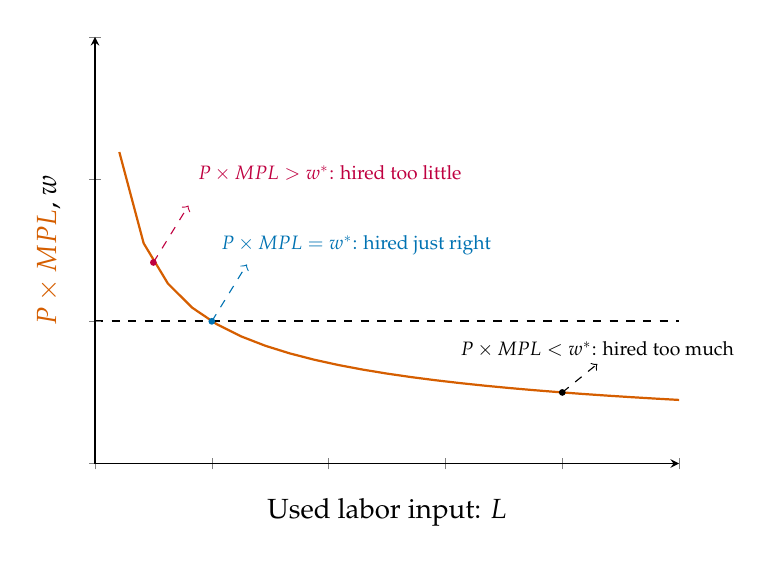
\begin{tikzpicture}
        \pgfmathsetmacro{\alpha}{0.5}    % preference for computers
        \pgfmathsetmacro{\K}{1}    % labor endowment
        \pgfmathsetmacro{\A}{1}    % labor endowment
        
        \centering
        \begin{axis}[
            ylabel={$\textcolor{red}{P \times MPL}$, $w$ },
            xlabel={Used labor input: $L$},
            ymin=0, ymax=1.5,
            xmin=0, xmax=5,
            yticklabel=\empty,
            xticklabel=\empty,
            axis lines=left,
            enlargelimits=false,
            clip=false,
            axis on top,
            scaled x ticks=false,
            width=9cm, height=7cm,
            title style={font=\bfseries}
        ]
        
        % PPF: Q_C = (L/a_C) - (a_R/a_C) * Q_R
        \addplot[thick, red, domain=0:5] {(1-\alpha)*\A*\K^(\alpha)/x^(\alpha)};
        
        
        \addplot[dashed, purple, ->] coordinates {(0.5  , {(1-\alpha)*\A*\K^(\alpha)/0.5^(\alpha)}) (0.5 + 0.3, {(1-\alpha)*\A*\K^(\alpha)/0.5^(\alpha)} + 0.2)};
        \addplot[mark=*, only marks, purple, mark size=1pt] coordinates {(0.5, {(1-\alpha)*\A*\K^(\alpha)/0.5^(\alpha)})};
        \node[anchor=south west, purple] at (axis cs:0.5 + 0.3, {(1-\alpha)*\A*\K^(\alpha)/0.5^(\alpha)} + 0.25) {\scriptsize $P\times MPL > w^*$: hired too little};
        
        \pgfmathsetmacro{\Lb}{((1-\alpha)* \A / 0.5)^(1/\alpha) * \K}    % labor endowment
        
        \addplot[dashed, blue, ->] coordinates {(\Lb, {(1-\alpha)*\A*\K^(\alpha)/\Lb^(\alpha)}) (\Lb + 0.3, {(1-\alpha)*\A*\K^(\alpha)/\Lb^(\alpha)} + 0.2)};
        \addplot[mark=*, only marks, blue, mark size=1pt] coordinates {(\Lb, {(1-\alpha)*\A*\K^(\alpha)/\Lb^(\alpha)})};
        \node[anchor=south west, blue] at (axis cs:0.5 + 0.5, {(1-\alpha)*\A*\K^(\alpha)/\Lb^(\alpha)} + 0.2) {\scriptsize $P\times MPL = w^*$: hired just right};
        
        
        \addplot[dashed, black, ->] coordinates {(4  , {(1-\alpha)*\A*\K^(\alpha)/4^(\alpha)}) (4 + 0.3, {(1-\alpha)*\A*\K^(\alpha)/4^(\alpha)} + 0.1)};
        \addplot[mark=*, only marks, black, mark size=1pt] coordinates {(4, {(1-\alpha)*\A*\K^(\alpha)/4^(\alpha)})};
        \node[black] at (axis cs:4 + 0.3, {(1-\alpha)*\A*\K^(\alpha)/4^(\alpha)}+0.15) {\scriptsize $P\times MPL < w^*$: hired too much};
        
        
        \addplot[thick, dashed, domain=0:5] {0.5};
        
        \end{axis}
        
        \end{tikzpicture}
        
              }
    }

\end{frame}

\begin{frame}{Solution to the Production Model}

Replacing the market clearing condition in and normalizing $P=1$ to be the num\'eraire of this economy:

  \begin{eqnarray}
    Y^* &=& \bar{Z} (\bar{K})^{\beta} (\bar{L})^{1-\beta} \\
    w^* &=& (1-\beta) \bar{Z} \left( \frac{\bar{K}}{\bar{L}} \right)^\beta  \\
     r^* &=&  \beta \bar{Z} \left( \frac{\bar{L}}{\bar{K}} \right)^{1-\beta}  \\
     L^* &=& \bar{L}  \\
     K^* &=& \bar{K}
  \end{eqnarray}

Note that everything on the right-hand side of the equations is a parameter, so this is indeed an explicit solution!
\end{frame}

\begin{frame}{Numerical Example}

Suppose $\bar{K} = 20, \bar{L} = 160, \bar{Z}=1, \beta=\frac{1}{3}$. What is the solution to the Production Model? Replacing in the set of equations before:

  \begin{eqnarray*}
    Y^* &=&  (20)^{\frac{1}{3}}  (160)^{\frac{2}{3}} = 80 \\
    w^* &=& \frac{2}{3} \left( \frac{20}{160} \right)^{\frac{1}{3}} = \frac{1}{3} \\
     r^* &=&  \frac{1}{3} \left( \frac{160}{20} \right)^{\frac{2}{3}} = \frac{4}{3}  \\
     L^* &=& 160  \\
     K^* &=& 20
  \end{eqnarray*}
\end{frame}


\begin{frame}{Solution to the Model in General Equilibrium}
\begin{figure}[htbp!]

\begin{subfigure}{}
\resizebox{0.48\textwidth}{!}{%
        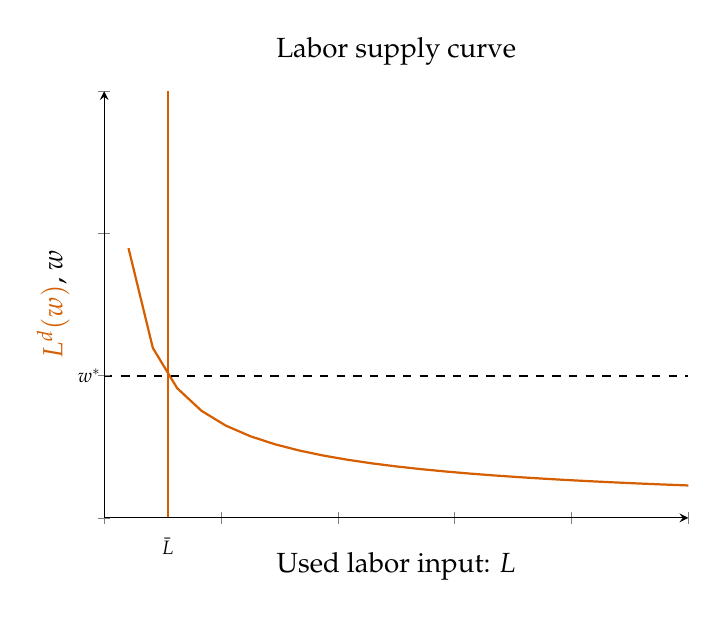
\begin{tikzpicture}
        \pgfmathsetmacro{\alpha}{2/3}
        \pgfmathsetmacro{\K}{1}
        \pgfmathsetmacro{\A}{1}
        
        \begin{axis}[
            ylabel={$\textcolor{red}{L^d(w)}$, $w$ },
            xlabel={Used labor input: $L$},
            ymin=0, ymax=1.5,
            xmin=0, xmax=5,
            yticklabel=\empty,
            xticklabel=\empty,
            axis lines=left,
            enlargelimits=false,
            clip=false,
            axis on top,
            scaled x ticks=false,
            width=9cm, height=7cm,
            title={Labor supply curve}
        ]
        \addplot[thick, red, domain=0:5] {(1-\alpha)*\A*\K^(\alpha)/x^(\alpha)};
        \addplot[thick, dashed, domain=0:5] {0.5};
        \addplot[thick, red] coordinates {({((1-\alpha)*\A/0.5)^(1/\alpha)*\K}, 1.5) ({((1-\alpha)*\A/0.5)^(1/\alpha)*\K},0)};

        %\node at (axis cs:3.5,0.03) {\Large $\mathcal{Y}_{US}$};
        \node at (axis cs:-0.125,0.5) {\scriptsize $w^*$};
        \node at (axis cs:({((1-\alpha)*\A/0.5)^(1/\alpha)*\K},-0.1) {\scriptsize $\bar{L}$};
        
        \end{axis}
        \end{tikzpicture}
}
\end{subfigure}
%
\begin{subfigure}{}
\resizebox{0.48\textwidth}{!}{%

        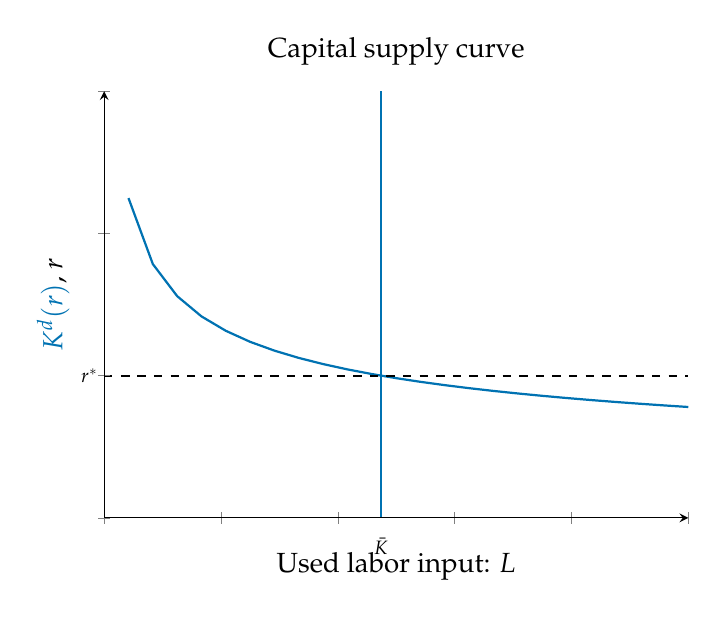
\begin{tikzpicture}
        \pgfmathsetmacro{\alpha}{1/3}
        \pgfmathsetmacro{\K}{1}
        \pgfmathsetmacro{\A}{1}
        
        \begin{axis}[
            ylabel={$\textcolor{blue}{K^d(r)}$, $r$ },
            xlabel={Used labor input: $L$},
            ymin=0, ymax=1.5,
            xmin=0, xmax=5,
            yticklabel=\empty,
            xticklabel=\empty,
            axis lines=left,
            enlargelimits=false,
            clip=false,
            axis on top,
            scaled x ticks=false,
            width=9cm, height=7cm,
            title={Capital supply curve}
        ]
        \addplot[thick, blue, domain=0:5] {(1-\alpha)*\A*\K^(\alpha)/x^(\alpha)};
        \addplot[thick, dashed, domain=0:5] {0.5};
        \addplot[thick, blue] coordinates {({((1-\alpha)*\A/0.5)^(1/\alpha)*\K}, 1.5) ({((1-\alpha)*\A/0.5)^(1/\alpha)*\K},0)};

        %\node at (axis cs:3.5,0.03) {\Large $\mathcal{Y}_{US}$};
        \node at (axis cs:-0.125,0.5) {\scriptsize $r^*$};
        \node at (axis cs:({((1-\alpha)*\A/0.5)^(1/\alpha)*\K},-0.1) {\scriptsize $\bar{K}$};
        \end{axis}
        \end{tikzpicture}
}

\end{subfigure}

\end{figure}
\end{frame}

\section{Specific Factors Model}

\begin{frame}
\addtocounter{framenumber}{-1}

\centering

\Huge{\blue{Specific Factors Model}}
    
\end{frame}

\begin{frame}{Specific Factors Model: Preliminaries}
    \begin{wideitemize}
        \item Number of factors of production: 3 (labor L, land T, capital K)
        
    \item Mobility of factors of production: Labor is mobile across sectors \\
    capital and land are sector specific (immobile)

    \item Number of sectors (goods): 2 
    \begin{itemize}
        \item Food output $Y_A$ uses $T$ and $L$
        \item Manufacturing output $Y_M$ uses $K$ and $L$
    \end{itemize}

    \item Perfect competition; no trade costs

    \item Key force: Differences in sector specific endowments
    \end{wideitemize}    
\end{frame}

\begin{frame}{Production}

    \begin{wideitemize}

        \item Production with sector-specific factors land \blue{$T$} and capital \blue{$K$}:
        \begin{eqnarray*}\label{eq: production}
            &\max_{L_{i,M}, \blue{K_{i}}}& P_{M} \times  Z_{i,M} \times \blue{K_{i}}^{\beta_i} L_{i,M}^{1-\beta_i} - w_i L_{i,M} - r_{i,M} K_{i} \\
            &\max_{L_{i,A}, \blue{T_{i}}}& P_{A} \times  Z_{i,A} \times \blue{T_{i}}^{\beta_i} L_{i,A}^{1-\beta_i} - w_i L_{i,A} - r_{i,A} T_{i} 
        \end{eqnarray*}

        \item Specific Factors model is also called the Ricardo-Viner model \\
        \begin{itemize}
            \item In common with Ricardo: Labor productivity differs across sectors
            \item Viner: Specific factor endowments determine labor productivity
            \item Implication: Unit labor requirements change with labor employment
        \end{itemize}
    \end{wideitemize}
\end{frame}

\begin{frame}{Optimality conditions}
\begin{wideitemize}
    
        \item At their optimal points, factor prices equal their marginal (revenue) product for labor...
        \begin{eqnarray*}
            P_M \times MPL_{i,M} = P_M \times  \frac{\partial Y_{i,M}}{\partial L_{i,M}} &=& w_i\\
            P_A \times MPL_{i,A} = P_A \times  \frac{\partial Y_{i,A}}{\partial L_{i,A}} &=& w_i 
        \end{eqnarray*}

        \item ... and for labor and capital, respectively:

                \begin{eqnarray*}
            P_M \times MPK_{i,M} =  P_M \times  \frac{\partial Y_{i,M}}{\partial K_{i,M}} &=&r_{i,M} \\
            P_A \times MPT_{i,A} = P_A \times  \frac{\partial Y_{i,A}}{\partial T_{i,A}} &=& r_{i,A}
        \end{eqnarray*}

\end{wideitemize}    
\end{frame}


\begin{frame}{Supply of Factors of Production}
\begin{wideitemize}
        \item Total labor can be distributed for the production of either good, such that:

        \begin{equation*}
            \underbrace{L_{i,A}}_{\substack{\text{labor used in} \\ \text{production of } A}} + \underbrace{L_{i,M}}_{\substack{\text{labor used in} \\ \text{production of } M}} \le \underbrace{L_i}_{\substack{\text{total labor} \\ \text{available in } i}}
        \end{equation*}

        \item Supply of land $T$ and capital is inelastic, so in equilibrium each sectors uses all endowment of specific factor:

        \begin{equation*}
            \underbrace{T_i}_{\substack{\text{land} \\ \text{demand}}} = \underbrace{\bar{T}_i}_{\substack{\text{land} \\ \text{supply}}}, \qquad              \underbrace{K_i}_{\substack{\text{capital} \\ \text{demand}}} = \underbrace{\bar{K}_i}_{\substack{\text{capital} \\ \text{supply}}} 
        \end{equation*}
\end{wideitemize}
\end{frame}

\begin{frame}{The economy in one diagram}
\addtocounter{framenumber}{-1}
\centering
    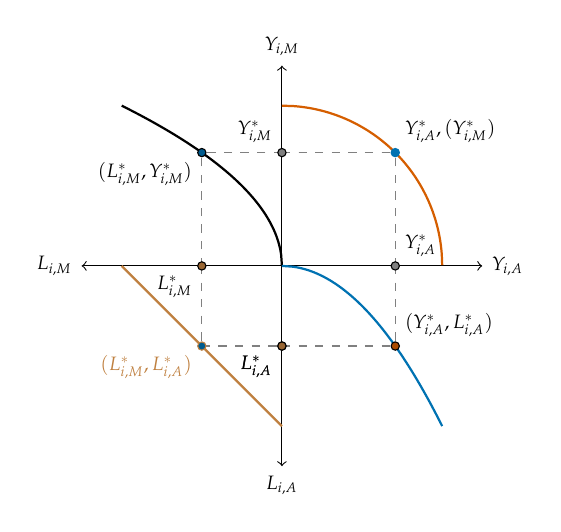
\begin{tikzpicture}
    \begin{axis}[
        axis lines=middle,
        xmin=-1.25, xmax=1.25,
        ymin=-1.25, ymax=1.25,
    %    xlabel={\small Output of cloth / Labor in cloth},
    %    ylabel={\small Output of food / Labor in food},
        xtick=\empty,
        ytick=\empty,
        axis line style={<->},
        clip=false,
        enlargelimits=false,
        domain=0.0:1,
        width=0.55\textwidth,
        height=0.55\textwidth,
        samples=200
    ]
    
    \pgfmathsetmacro{\a}{0.5}       % curvature parameter
    
    % NW: Production function for food (plot in 2nd quadrant)
    \addplot[black, thick] ({-x}, {x^(\a)});
    \node[anchor=east] at (axis cs:-1.25,0) {\scriptsize $L_{i,M}$};
    \node[anchor=south] at (axis cs:0,1.25) {\scriptsize $Y_{i,M}$};
    
    % SW: Labor allocation AA curve (line in 3rd quadrant)
    \addplot[brown, thick] ({-x}, {-1 + x});
    %\node[anchor=north east] at (axis cs:-0.95,-0.05) {\scriptsize Economy's allocation of labor (AA)};
    
    % SE: Production function for cloth (4th quadrant)
    \addplot[blue, thick] ({x^(\a)}, {-x});
    \node[anchor=west] at (axis cs:1.25,0) {\scriptsize $Y_{i,A}$};
    \node[anchor=north] at (axis cs:0,-1.25) {\scriptsize $L_{i,A}$};
    %\node[anchor=north west] at (axis cs:0.6,-0.6) {\scriptsize Production function for cloth};
    
    % NE: Production Possibility Frontier (PPF)
    \addplot[red, thick] ({x^(\a)}, {(1 - x)^(\a)});
    %\node[anchor=south east, blue] at (axis cs:0.6,0.65) {\scriptsize $PP$};
    
    % point on AA
    \addplot+[mark=*,only marks,mark size=1.5pt,brown]
                  coordinates {({-0.5},{-1+0.5})}
                  node[anchor=north east,font=\scriptsize, brown] {$(L_{i,M}^*,L_{i,A}^*)$};
    
    \addplot[dashed, gray] coordinates {({-0.5}, {-1 + 0.5}) (0, {-1 + 0.5})};

    \addplot+[mark=*,only marks,mark size=1.5pt,black]
                  coordinates {({-0.5}, 0)}
                  node[anchor=north east,font=\scriptsize] {$L_{i,M}^*$};

        \addplot+[mark=*,only marks,mark size=1.5pt,black]
                  coordinates {(0, {0.5^(\a)})}
                  node[anchor=south east,font=\scriptsize] {$Y_{i,M}^*$};

    % Project to NW (Food PF)
    \addplot[dashed, gray] coordinates {({-0.5}, 0) ({-0.5}, {0.5^(\a)})};
    \addplot[dashed, gray] coordinates {(0, {0.5^(\a)}) ({-0.5},{0.5^(\a)})};
    \addplot+[mark=*, only marks, mark size=1.5pt, black]
            coordinates {({-0.5}, {0.5^(\a)})}
            node[anchor=north east, font=\scriptsize]{$(L_{i,M}^*,Y_{i,M}^*)$};     

    \addplot[dashed, gray] coordinates {({-0.5}, 0) ({-0.5}, {-(1-0.5)})};
    \addplot+[mark=*,only marks,mark size=1.5pt,black]
                  coordinates { (0, {-(1-0.5)})}
                  node[anchor=north east,font=\scriptsize] {$L_{i,A}^*$};

        % Project to SE (Cloth PF)
    \addplot[dashed, gray] coordinates {(0, {-0.5}) ({0.5^(\a)}, {-0.5})};
    \addplot[dashed, gray] coordinates {({0.5^(\a)}, 0) ({0.5^(\a)}, {-0.5})};
    \addplot+[mark=*, only marks, mark size=1.5pt, black]
            coordinates {({0.5^(\a)}, {-0.5})}
            node[anchor=south west,font=\scriptsize] {$(Y_{i,A}^*,L_{i,A}^*)$};
    
    \addplot+[mark=*,only marks,mark size=1.5pt,black]
                  coordinates { (0, {-(1-0.5)})}
                  node[anchor=north east,font=\scriptsize] {$L_{i,A}^*$};

        \addplot+[mark=*,only marks,mark size=1.5pt,black]
                  coordinates {({0.5^(\a)},0)}
                  node[anchor=south west,font=\scriptsize] {$Y_{i,A}^*$};


    % Project to NE (PPF)
    \pgfmathsetmacro{\Qc}{0.5^(\a)}
    \pgfmathsetmacro{\Qf}{(1 - 0.5)^(\a)}
    \addplot+[mark=*, only marks, mark size=1.5pt]
            coordinates {(\Qc, \Qf)}
            node[anchor=south west, font=\scriptsize, black]{$Y_{i,A}^*,(Y_{i,M}^*)$};     
    \addplot[dashed, gray] coordinates {(\Qc, 0) (\Qc, \Qf)};
    \addplot[dashed, gray] coordinates {(0, \Qf) (\Qc, \Qf)};
    \addplot[dashed, gray] coordinates {(0, \Qf) (\Qc, \Qf)};

    
    \end{axis}
    
    \end{tikzpicture}
\end{frame}



\begin{frame}{Labor Market Equilibrium: Intuition}
\begin{wideitemize}
    \item Recall the labor market resource constraint:
        \begin{equation*}
            L_{i,A} + L_{i,M} = \bar{L}_{i} \iff L_{i,M} = \bar{L}_{i} - L_{i,A}  
        \end{equation*}

    \item In other words, labor is either allocated to manufacturing or to agriculture (trade off)

    \item  Also, recall the equilibrium condition for labor:

            \begin{eqnarray*}
            P_M \times MPL_{i,M} = P_M \times  \frac{\partial Y_{i,M}}{\partial L_{i,M}} &=& w_i\\
            P_A \times MPL_{i,A} = P_A \times  \frac{\partial Y_{i,A}}{\partial L_{i,A}} &=& w_i  
        \end{eqnarray*}

    \item Implication: equilibrium wage $w_i^*$ will be the point that equalizes marginal revenue 

    \begin{equation*}
        P_M \times MPL_{i,M}  =  P_A \times MPL_{i,A}
    \end{equation*}

\end{wideitemize}
    
\end{frame}

\begin{frame}{Labor Market Equilibrium: Numerical Example}
    \begin{wideitemize}
        \item Suppose $Z_{i,A} = 1$, $T_i = 4$, $Z_{i,M} = 4$, $K_i = 1$, $P_M=1$, $P_A=2$, $\beta_i=1/2$, $\bar{L}_i=1$. Solve for $\{L_M,L_A,w_{i}^*\}$
    { \scriptsize
    \begin{eqnarray*}
        P_{M} \times  MPL_{i,M} = P_{M} \times  Z_{i,M} \times (1-\beta_i) \times \left( \frac{K_{i}}{L_{i,M}} \right)^{\beta_i} &=& 1 \times  4 \times \frac{1}{2} \times \left( \frac{1}{L_{i,M}} \right)^{1/2} =  \frac{2}{\sqrt{ L_{i,M}}} \\
        P_{A} \times  MPL_{i,A} = P_{A} \times  Z_{i,A} \times (1-\beta_i) \times \left( \frac{T_{i}}{\bar{L}_i - L_{i,M}} \right)^{\beta_i} &=& 2 \times  1 \times \frac{1}{2} \times \left( \frac{4}{1 - L_{i,M}} \right)^{1/2} =  \frac{\sqrt{4}}{\sqrt{1 - L_{i,M}}} =  \frac{2}{\sqrt{1 - L_{i,M}}} 
    \end{eqnarray*}
    }
    \item<2-> Then:
{ \footnotesize
    \begin{equation*}
         P_{M} \times  MPL_{i,M} = \frac{2}{\sqrt{ L_{i,M}}} = \frac{2}{\sqrt{1 - L_{i,M}}} = P_{A} \times  MPL_{i,A} \iff L_{i,M} = 1 - L_{i,M} \iff L_{i,M} = \frac{1}{2}   
    \end{equation*}
     }

    \item<3-> To find wage:
    \begin{equation*}
        w_i = P_{i,M} \times MPL_{i,M} = \frac{2}{\sqrt{ L_{i,M}}}  = \frac{2}{\sqrt{  \frac{1}{2} }} = 2\sqrt{2}
    \end{equation*} 
    \end{wideitemize}

\end{frame}

\begin{frame}{Labor Market Equilibrium: General Case}
    \begin{wideitemize}
        \item What is $\Omega_i = \left( \frac{P_{M} \times  Z_{i,M}}{P_{A} \times  Z_{i,A}} \right)^{\frac{1}{\beta_i}} \times  \frac{K_{i}}{T_{i}}$? This term reflects: 
        \begin{itemize}
            \item relative profitability and tech, scaled by how responsive production is to labor (via $\beta_i$); and
            \item relative capacity of the two sectors to employ labor, given the specific factors ($K_i$, $T_i$).
        \end{itemize}
        \item<2-> Then:
        \begin{equation*}
         \Omega_i \times (\bar{L}_i - L_{i,M}) =  L_{i,M} \iff  L_{i,M} = \frac{\Omega_i}{1+\Omega_i} \times \bar{L}_i
         \end{equation*}
         \item<3-> ...and:
        \begin{equation*}
           L_{i,A} = \bar{L}_i - L_{i,M} =  \frac{1}{1+\Omega_i}  \times  \bar{L}_i
        \end{equation*}

        \item<4-> Note: $L_{i,M} / L_{i,A} = \Omega_i$
        \qquad (parameters in $\Omega_i$ pin down relative labor allocation) 
        
    \end{wideitemize}
\end{frame}




\begin{frame}{Labor Market Equilibrium: Diagram}
\addtocounter{framenumber}{-1}

\begin{figure}
    \centering
    \begin{tikzpicture}
    
    % Setup axis
    \begin{axis}[
        axis lines=middle,
        xtick=\empty,
        ytick=\empty,
        xmin=0, xmax=2.2,
        ymin=0, ymax=1.2,
        samples=300,
        axis line style={->},
        width=12cm,
        height=8cm,
        domain=0.05:1.05,
        clip=false,
    ]
    
    \pgfmathsetmacro{\Pm}{1}
    \pgfmathsetmacro{\beta}{0.5}
    \pgfmathsetmacro{\Zm}{1}
    \pgfmathsetmacro{\K}{1}
    
    \pgfmathsetmacro{\Pa}{1}
    \pgfmathsetmacro{\beta}{0.5}
    \pgfmathsetmacro{\Za}{1}
    \pgfmathsetmacro{\T}{1}
    
    \pgfmathsetmacro{\Omega}{(\Pm*\Zm / \Pa*\Za)^(1/\beta) * \K / \T}
    \pgfmathsetmacro{\L}{2.2}
    
    \pgfmathsetmacro{\Ls}{ \Omega / (1+\Omega) * \L}
    \pgfmathsetmacro{\ws}{ \Pm * \Zm * (1-\beta) * (\K / \Ls )^(\beta) }
    
    
    
    
    \addplot[->] coordinates {(2.2,0) (2.2,1.2)};
    \addplot[->] coordinates {(2.2,0) (0,0)};
    
    
    % Demand in manufacturing (left)
    \addplot[domain=0.2:2.2, thick, red] (x, {\Pm * \Zm * (1-\beta) * (\K / x)^(\beta)});
    \node[align=center, anchor=north west, red!70] at (axis cs:0.2,0.65) {\small $P_M \times MPL_{i,M}$};
    \node[black, P] at (axis cs:-0.25,1.15) {\scriptsize $w_i$, \textcolor{red}{$P_M \times MPL_{i,M}$}};
    \node[black] at (axis cs:0,-0.04) {\scriptsize $0~(\bar{L}_i)$};
    
    % Demand in food (right)
    \addplot[domain=0.2:2.2, thick, blue] (2.2-x, {(\Pa * \Za * (1-\beta) * (\T / x)^(\beta)});
    \node[align=center, anchor=north east, blue!70] at (axis cs:2.2-0.2,0.65) {\small $P_A \times MPL_{i,A}$};
    \node[black, P] at (axis cs:2.2+0.25,1.15) {\scriptsize $w_i$, \textcolor{blue}{$P_A \times MPL_{i,A}$}};
    \node[black] at (axis cs:2.2,-0.04) {\scriptsize $\bar{L}_i~(0)$};
    
    % Equilibrium point
    \addplot[dashed] coordinates {(0,\ws) (2.2,\ws)};
    \addplot[mark=*, black, mark size=1.5pt] coordinates {(\Ls,\ws)};
    \addplot[dashed] coordinates {(\Ls,0) (\Ls,\ws)};
    \node[below] at (axis cs:\Ls,-0.02) {\small $L_M = \bar{L} - L_A$};
    \node[black, P] at (axis cs:-0.05,\ws) {\scriptsize $w_i^*$};
    \node[black, P] at (axis cs:2.2+0.05,\ws) {\scriptsize $w_i^*$};
    
    % Bottom left and right axis labels
    %\node[below] at (axis cs:-0.5,-0.02) {\scriptsize $L_M$};
    %\node[below] at (axis cs:0.5,-0.02) {\scriptsize $L - L_M~(= L_F)$};
    
    \end{axis}
    
    \end{tikzpicture}
\end{figure}

\end{frame}

\begin{frame}{Distribution of income: Diagram}

\begin{figure}[htp]
    \centering
    \begin{tikzpicture}
    
    % Setup axis
    \begin{axis}[
        axis lines=middle,
        xtick=\empty,
        ytick=\empty,
        xmin=0, xmax=2.2,
        ymin=0, ymax=1.2,
        samples=300,
        axis line style={->},
        width=12cm,
        height=8cm,
        domain=0.05:1.05,
        clip=false,
    ]
    
    \pgfmathsetmacro{\Pm}{1}
    \pgfmathsetmacro{\beta}{0.5}
    \pgfmathsetmacro{\Zm}{1}
    \pgfmathsetmacro{\K}{1}
    
    \pgfmathsetmacro{\Pa}{1}
    \pgfmathsetmacro{\beta}{0.5}
    \pgfmathsetmacro{\Za}{1}
    \pgfmathsetmacro{\T}{1}
    
    \pgfmathsetmacro{\Omega}{(\Pm*\Zm / \Pa*\Za)^(1/\beta) * \K / \T}
    \pgfmathsetmacro{\L}{2.2}
    
    \pgfmathsetmacro{\Ls}{ \Omega / (1+\Omega) * \L}
    \pgfmathsetmacro{\ws}{ \Pm * \Zm * (1-\beta) * (\K / \Ls )^(\beta) }
    
    
    
    
    \addplot[->] coordinates {(2.2,0) (2.2,1.2)};
    \addplot[->] coordinates {(2.2,0) (0,0)};
    
    
    % Demand in manufacturing (left)
    \addplot[domain=0.2:2.2, thick, red] (x, {\Pm * \Zm * (1-\beta) * (\K / x)^(\beta)});
    \node[align=left, anchor=north west, red!70] at (axis cs:0.2,0.65) {\scriptsize Manufacturing \\ \scriptsize producers income };
    \node[black, P] at (axis cs:-0.25,1.15) {\scriptsize $w_i$, \textcolor{red}{$P_M \times MPL_{i,M}$}};
    \node[black] at (axis cs:0,-0.04) {\scriptsize $0~(\bar{L}_i)$};

    % Demand in food (right)
    \addplot[domain=0.2:2.2, thick, blue] (2.2-x, {(\Pm * \Zm * (1-\beta) * (\K / x)^(\beta)});
    \node[align=right, anchor=north east, blue!70] at (axis cs:2.2-0.2,0.65) {\scriptsize Agricultural \\ \scriptsize producers income };
    \node[black, P] at (axis cs:2.2+0.25,1.15) {\scriptsize $w_i$, \textcolor{blue}{$P_A \times MPL_{i,A}$}};
    \node[black] at (axis cs:2.2,-0.04) {\scriptsize $\bar{L}_i~(0)$};
    
    % Equilibrium point
    \addplot[dashed] coordinates {(0,\ws) (2.2,\ws)};
    \addplot[mark=*, black, mark size=1.5pt] coordinates {(\Ls,\ws)};
    \addplot[dashed] coordinates {(\Ls,0) (\Ls,\ws)};
    \node[below] at (axis cs:\Ls,-0.02) {\small $L_M = \bar{L} - L_A$};
    \node[black, P] at (axis cs:-0.05,\ws) {\scriptsize $w_i^*$};
    \node[black, P] at (axis cs:2.2+0.05,\ws) {\scriptsize $w_i^*$};  
    \node[align=center, anchor=north, black!70] at (axis cs:1.1,0.35) {\small Workers' \text{      } income};

    % Fillings
        % manufacturing producer
        \addplot [
        name path=A,
        domain=0.2:\Ls,
        draw=none
        ] (x, {\Pm * \Zm * (1-\beta) * (\K / x)^(\beta)});
    
        \path[name path=B] (axis cs:0.2,\ws) -- (axis cs:\Ls,\ws);
    
        \addplot [
            fill=red!20,
            draw=none
            ] fill between [of=A and B];

        % agricultural producer
        \addplot [
        name path=C,
        domain=0.2:\Ls,
        draw=none
        ] (2.2-x, {(\Pm * \Zm * (1-\beta) * (\K / x)^(\beta)});
    
        \path[name path=D] (axis cs:\Ls,\ws) -- (axis cs:2.2-0.2,\ws);
    
        \addplot [
            fill=blue!20,
            draw=none
            ] fill between [of=C and D];

        % workers
        \addplot [
        name path=E,
        domain=0.2:2,
        draw=none
        ] (x,\ws);
    
        \path[name path=F] (axis cs:0.2,0) -- (axis cs:2.2-0.2,0);
    
        \addplot [
            fill=black!20,
            draw=none
            ] fill between [of=E and F];


    \end{axis}
    \end{tikzpicture}
\end{figure}
    
\end{frame}

\begin{frame}{Autarky Equilibrium: Intuition}
\begin{figure}
    \centering
        \begin{tikzpicture}
        
    \pgfmathsetmacro{\beta}{1/3}
    \pgfmathsetmacro{\alpha}{2/3}

    \pgfmathsetmacro{\Zm}{1}
    \pgfmathsetmacro{\K}{1}
    
    \pgfmathsetmacro{\Za}{1}
    \pgfmathsetmacro{\T}{1}

    \pgfmathsetmacro{\Ps}{\Za/\Zm * ((1-\alpha)/\alpha * \T / \K  )^(\beta)}
    
    \pgfmathsetmacro{\Qs}{(1-\alpha)/\alpha / \Ps}

    
    

        \centering
        \begin{axis}[
            ylabel={Relative price $P_M / P_A$ },
            xlabel={Relative Quantity: \textcolor{red}{$Q_{i,M}/Q_{i,A}$}, \textcolor{blue}{$Y_{i,M}/Y_{i,A}$}},
            ymin=0, ymax=3,
            xmin=0, xmax=2,
            yticklabel=\empty,
            xticklabel=\empty,
            axis lines=left,
            enlargelimits=false,
            clip=false,
            axis on top,
            scaled x ticks=false,
            width=9cm, height=7cm,
            title style={font=\bfseries}
        ]
        
        % demand
        \addplot[domain=0.4:1.7, thick, red] (x, {(1-\alpha)/\alpha / x});
        % supply
        \addplot[domain=0.2:1.3, thick, blue] ({(\Zm/\Za)^(1/\beta) * ( \K / \T ) * x^((1-\beta)/\beta)}, x);
        
        \addplot[dashed] coordinates {(0,\Ps) (\Qs,\Ps)};
        \node[blac] at (axis cs:-0.1,\Ps) {\small $\frac{P_{M}^*}{P_{A}^*}$};
        \addplot[dashed] coordinates {(\Qs,\Ps) (\Qs,0)};
         \node[blac] at (axis cs:\Qs,-0.2) {\small $\textcolor{red}{RD_i} = \textcolor{blue}{RS_i}$};

        
        %\addplot[thick, dashed, domain=0:5] {0.5};
        
        \end{axis}
        
        \end{tikzpicture}
        \caption{Relative Supply and Relative Demand as functions of relative prices}
    \label{fig: rd-rs-autarky}
\end{figure}

\end{frame}

\begin{frame}{Trade Equilibrium: Global Demand and Supply}
\begin{figure}
    \centering
        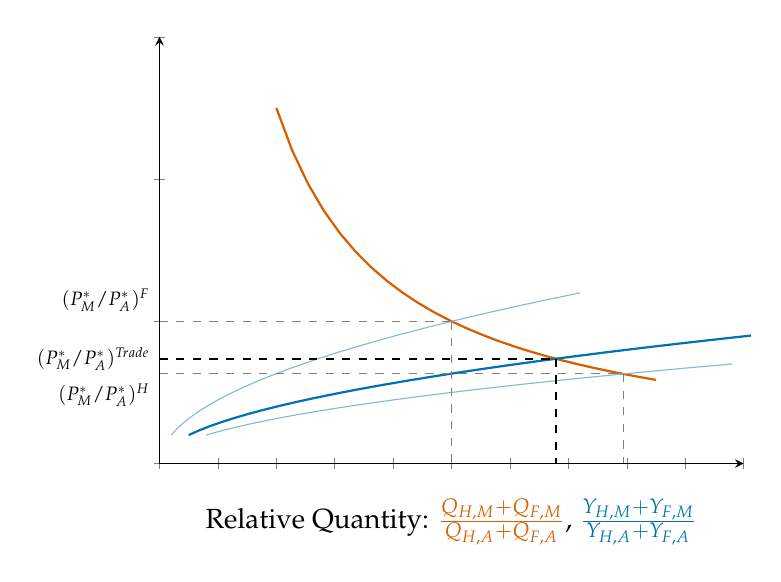
\begin{tikzpicture}
        
    \pgfmathsetmacro{\beta}{1/3}
    \pgfmathsetmacro{\alpha}{0.5}

    \pgfmathsetmacro{\Zm}{1}
    \pgfmathsetmacro{\K}{4}
    
    \pgfmathsetmacro{\Za}{1}
    \pgfmathsetmacro{\T}{1}

    \pgfmathsetmacro{\Kf}{1}
    \pgfmathsetmacro{\Tf}{1}


    \pgfmathsetmacro{\Ps}{\Za/\Zm * ((1-\alpha)/\alpha * \T / \K)^(\beta)}   
    \pgfmathsetmacro{\Qs}{(1-\alpha)/\alpha / \Ps}

    \pgfmathsetmacro{\Psf}{\Za/\Zm * ((1-\alpha)/\alpha * \Tf / \Kf)^(\beta)}   
    \pgfmathsetmacro{\Qsf}{(1-\alpha)/\alpha / \Psf}

    \pgfmathsetmacro{\Psw}{\Za/\Zm * ((1-\alpha)/\alpha * ( ( \T + \Tf) / (\K+\Kf ) )^(\beta)}   
    \pgfmathsetmacro{\Qsw}{(1-\alpha)/\alpha / \Psw}

    
    

        \centering
        \begin{axis}[
            xlabel={Relative Quantity: \textcolor{red}{$\frac{Q_{H,M} + Q_{F,M}}{Q_{H,A} + Q_{F,A}}$}, \textcolor{blue}{$\frac{Y_{H,M} + Y_{F,M}}{Y_{H,A} + Y_{F,A}}$}},
            ymin=0, ymax=3,
            xmin=0, xmax=2,
            yticklabel=\empty,
            xticklabel=\empty,
            axis lines=left,
            enlargelimits=false,
            clip=false,
            axis on top,
            scaled x ticks=false,
            width=9cm, height=7cm,
            title style={font=\bfseries}
        ]
        
        % demand
        \addplot[domain=0.4:1.7, thick, red] (x, {(1-\alpha)/\alpha / x});
        % supply home
        \addplot[domain=0.2:0.7, blue!50] ({(\Zm/\Za)^(1/\beta) * ( \K / \T ) * x^((1-\beta)/\beta)}, x);
        % supply foreign
        \addplot[domain=0.2:1.2, blue!50] ({(\Zm/\Za)^(1/\beta) * ( \Kf / \Tf ) * x^((1-\beta)/\beta)}, x);
        % supply world
        \addplot[domain=0.2:0.9, thick, blue] ({(\Zm/\Za)^(1/\beta) * ( (\K+\Kf) / (\T+\Tf) ) * x^((1-\beta)/\beta)}, x);
        %\addplot[domain=0.2:1.3, thick, blue] (x, {(\Zm/\Za)^(- 1/\beta) * x^((1-\beta)/\beta) * ( (\Kf + \K) / ( \Tf + \T ) ) });
        
        \addplot[dashed, gray] coordinates {(0,\Ps) (\Qs,\Ps)};
        \node[black, anchor=north east] at (axis cs:0,\Ps) {\scriptsize $(P_{M}^*/P_{A}^*)^H$};
        \addplot[dashed, gray] coordinates {(\Qs,\Ps) (\Qs,0)};

        \addplot[dashed, gray] coordinates {(0,\Psf) (\Qsf,\Psf)};
        \node[black, anchor=south east] at (axis cs:0,\Psf) {\scriptsize $(P_{M}^*/P_{A}^*)^F$};
        \addplot[dashed, gray] coordinates {(\Qsf,\Psf) (\Qsf,0)};

        \addplot[dashed, thick] coordinates {(0,\Psw) (\Qsw,\Psw)};
        \node[black, anchor=east] at (axis cs:0,\Psw) {\scriptsize $(P_{M}^*/P_{A}^*)^{Trade}$};
        \addplot[dashed, thick] coordinates {(\Qsw,\Psw) (\Qsw,0)};

        %\addplot[dashed] coordinates {(0,\Psw) (\Qsw,\Psw)};
        %\node[black] at (axis cs:-0.1,\Psw) {\small $(P_{M}^*/P_{A}^*)^{Trade}$};
        %\addplot[dashed] coordinates {(\Qsw,\Psw) (\Qsw,0)};
        % \node[black] at (axis cs:\Qs,-0.15) {\small $\textcolor{red}{RD_i} = \textcolor{blue}{RS_i}$};

        
        %\addplot[thick, dashed, domain=0:5] {0.5};
        
        \end{axis}
        
        \end{tikzpicture}
        \caption{World Trade Equilibrium}
    \label{fig: trade-eqm}
\end{figure}
\end{frame}

\begin{frame}{Trade Equilibrium: Implications for Production}
\begin{wideitemize}
    \item Capital is more abundant at home, so in autarky prices of manufacturing are low
    
    \item After trade, relative price of manufacturing increases
    

    \begin{equation*}
        (P_{M}/P_{A})^{H} < (P_{M}/P_{A})^{Trade} < (P_{M}/P_{A})^{F}
    \end{equation*}

    \item Home shifts production towards manufacturing (comparative advantage)
    
    \item Home uses higher price to expand consumption (gains from trade)
        
\end{wideitemize}
\end{frame}

\begin{frame}{Gains from trade at home}

\begin{figure}
    \centering
    \begin{tikzpicture}
    \pgfmathsetmacro{\beta}{1/3}
    \pgfmathsetmacro{\alpha}{0.5}

    \pgfmathsetmacro{\Zm}{1}
    \pgfmathsetmacro{\K}{1}
    
    \pgfmathsetmacro{\Za}{1}
    \pgfmathsetmacro{\T}{1}

    \pgfmathsetmacro{\Kf}{1}
    \pgfmathsetmacro{\Tf}{15}


    \pgfmathsetmacro{\P}{\Za/\Zm * ((1-\alpha)/\alpha * \T / \K)^(\beta)}   


    \pgfmathsetmacro{\Pw}{\Za/\Zm * ((1-\alpha)/\alpha * ( ( \T + \Tf) / (\K+\Kf ) )^(\beta)}  
    \pgfmathsetmacro{\Qw}{(1-\alpha)/\alpha / \Pw}

    \pgfmathsetmacro{\L}{1}
    \pgfmathsetmacro{\Omega}{(\P *\Zm / \Za)^(1/\beta) * \K / \T}      
    \pgfmathsetmacro{\Ls}{ \Omega / (1+\Omega) * \L}    
    \pgfmathsetmacro{\Ym}{ \Zm * \K^(\beta) * \Ls^(1-\beta) }
    \pgfmathsetmacro{\Ya}{ \Za * \T^(\beta) * (1-\Ls)^(1-\beta) }

    \pgfmathsetmacro{\Omegaw}{(\Pw *\Zm / \Za)^(1/\beta) * \K / \T}      
    \pgfmathsetmacro{\Lsw}{ \Omegaw / (1+\Omegaw) * \L}    
    \pgfmathsetmacro{\Ymw}{ \Zm * \K^(\beta) * \Lsw^(1-\beta) }
    \pgfmathsetmacro{\Yaw}{ \Za * \T^(\beta) * (1-\Lsw)^(1-\beta) }
    \pgfmathsetmacro{\Iw}{ \Pw * \Ymw + \Yaw }
    \pgfmathsetmacro{\Qaw}{(1-\alpha) * \Iw}
    \pgfmathsetmacro{\Qmw}{(\alpha)/\Pw * \Iw}

%    \pgfmathsetmacro{\ws}{ \Pm * \Zm * (1-\beta) * (\K / \Ls )^(\beta) }   
    % Compute utility level
    \pgfmathsetmacro{\U}{(\Ya^(\alpha))*(\Ym^(1 - \alpha))}
    \pgfmathsetmacro{\Uw}{(\Qaw^(\alpha))*(\Qmw^(1 - \alpha))}
    
    % Compute prefactor for indifference curve: Qc = A * Qr^(- (1 - alpha)/alpha)
    \pgfmathsetmacro{\expo}{\alpha/(1 - \alpha)}
    \pgfmathsetmacro{\A}{\U^(1/\alpha)}
    \pgfmathsetmacro{\Aw}{\Uw^(1/\alpha)}
    
    \centering
    \begin{axis}[
        xlabel={Quantity of manufacturing, $\textcolor{red}{Q_{i,M}}, \textcolor{blue}{Y_{i,M}}$},
        ylabel={Quantity of food, $\textcolor{red}{Q_{i,A}}, \textcolor{blue}{Y_{i,A}}$},
        ymin=0, ymax=\L+.5,
        xmin=0, xmax=\L+.5,
        yticklabel=\empty,
        xticklabel=\empty,
        axis lines=left,
        enlargelimits=false,
        clip=false,
        axis on top,
        scaled x ticks=false,
        width=9cm, height=6cm,
        title style={font=\bfseries}
    ]
    
    % PPF: Q_C = (L/a_C) - (a_R/a_C) * Q_R
    \addplot[blue, thick, domain=0:1] ({ \Zm * \K^(\beta) * (\L-x)^(1-\beta)}, {\Za * \T^(\beta) * (x)^(1-\beta)});
    \pgfmathsetmacro{\c}{ \Ym + \P * \Ya }
    \addplot[thick, brown, domain=0.2:1.2] { \c - \P*x};

    \addplot[thick, red, domain=0.3:1.2, samples=100] {\A * x^(-\expo)};
    
    % Labels
    %\node at (axis cs:3.5,0.03) {\Large $\mathcal{Y}_{US}$};
    %\node at (axis cs:\Lendow/\aR,-.01) {\scriptsize $\frac{L_{US}}{a_{US,R}}$};
    %\node at (axis cs:-.75,\Lendow/\aC) {\scriptsize $\frac{L_{US}}{a_{US,C}}$};
    
    
    % Equilibrium point
    \addplot[only marks, mark=*, color=bkacj, mark size=2pt] coordinates {(\Ym, \Ya)};
    
   
    
    \end{axis}
    \end{tikzpicture}
    
    \caption{Optimal Consumption and Production Choices for Society as a Whole}
    \label{fig: consumption-trade}
\end{figure}
\end{frame}

\begin{frame}{Gains from trade at home}
\addtocounter{framenumber}{-1}

\begin{figure}
    \centering
    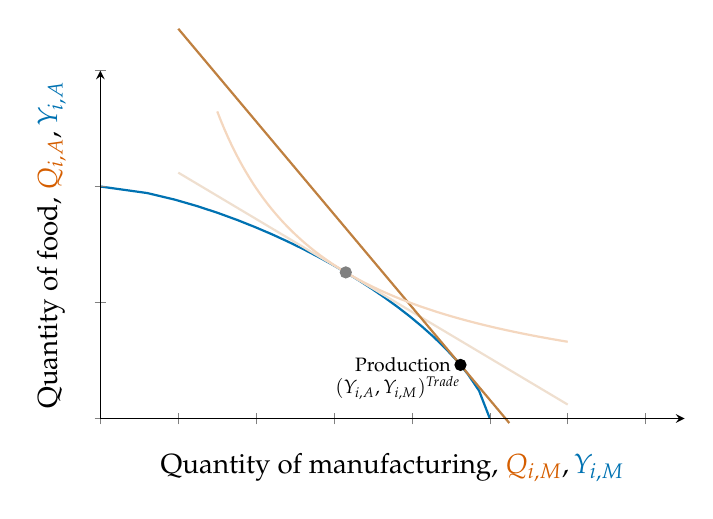
\begin{tikzpicture}
    \pgfmathsetmacro{\beta}{1/3}
    \pgfmathsetmacro{\alpha}{0.5}

    \pgfmathsetmacro{\Zm}{1}
    \pgfmathsetmacro{\K}{1}
    
    \pgfmathsetmacro{\Za}{1}
    \pgfmathsetmacro{\T}{1}

    \pgfmathsetmacro{\Kf}{1}
    \pgfmathsetmacro{\Tf}{15}


    \pgfmathsetmacro{\P}{\Za/\Zm * ((1-\alpha)/\alpha * \T / \K)^(\beta)}   


    \pgfmathsetmacro{\Pw}{\Za/\Zm * ((1-\alpha)/\alpha * ( ( \T + \Tf) / (\K+\Kf ) )^(\beta)}  
    \pgfmathsetmacro{\Qw}{(1-\alpha)/\alpha / \Pw}

    \pgfmathsetmacro{\L}{1}
    \pgfmathsetmacro{\Omega}{(\P *\Zm / \Za)^(1/\beta) * \K / \T}      
    \pgfmathsetmacro{\Ls}{ \Omega / (1+\Omega) * \L}    
    \pgfmathsetmacro{\Ym}{ \Zm * \K^(\beta) * \Ls^(1-\beta) }
    \pgfmathsetmacro{\Ya}{ \Za * \T^(\beta) * (1-\Ls)^(1-\beta) }

    \pgfmathsetmacro{\Omegaw}{(\Pw *\Zm / \Za)^(1/\beta) * \K / \T}      
    \pgfmathsetmacro{\Lsw}{ \Omegaw / (1+\Omegaw) * \L}    
    \pgfmathsetmacro{\Ymw}{ \Zm * \K^(\beta) * \Lsw^(1-\beta) }
    \pgfmathsetmacro{\Yaw}{ \Za * \T^(\beta) * (1-\Lsw)^(1-\beta) }
    \pgfmathsetmacro{\Iw}{ \Pw * \Ymw + \Yaw }
    \pgfmathsetmacro{\Qaw}{(1-\alpha) * \Iw}
    \pgfmathsetmacro{\Qmw}{(\alpha)/\Pw * \Iw}

%    \pgfmathsetmacro{\ws}{ \Pm * \Zm * (1-\beta) * (\K / \Ls )^(\beta) }   
    % Compute utility level
    \pgfmathsetmacro{\U}{(\Ya^(\alpha))*(\Ym^(1 - \alpha))}
    \pgfmathsetmacro{\Uw}{(\Qaw^(\alpha))*(\Qmw^(1 - \alpha))}
    
    % Compute prefactor for indifference curve: Qc = A * Qr^(- (1 - alpha)/alpha)
    \pgfmathsetmacro{\expo}{\alpha/(1 - \alpha)}
    \pgfmathsetmacro{\A}{\U^(1/\alpha)}
    \pgfmathsetmacro{\Aw}{\Uw^(1/\alpha)}
    
    \centering
    \begin{axis}[
        xlabel={Quantity of manufacturing, $\textcolor{red}{Q_{i,M}}, \textcolor{blue}{Y_{i,M}}$},
        ylabel={Quantity of food, $\textcolor{red}{Q_{i,A}}, \textcolor{blue}{Y_{i,A}}$},
        ymin=0, ymax=\L+.5,
        xmin=0, xmax=\L+.5,
        yticklabel=\empty,
        xticklabel=\empty,
        axis lines=left,
        enlargelimits=false,
        clip=false,
        axis on top,
        scaled x ticks=false,
        width=9cm, height=6cm,
        title style={font=\bfseries}
    ]
    
    % PPF: Q_C = (L/a_C) - (a_R/a_C) * Q_R
    \addplot[blue, thick, domain=0:1] ({ \Zm * \K^(\beta) * (\L-x)^(1-\beta)}, {\Za * \T^(\beta) * (x)^(1-\beta)});
    \pgfmathsetmacro{\c}{ \Ym + \P * \Ya }
    \addplot[thick, brown!25, domain=0.2:1.2] { \c - \P*x};

    \pgfmathsetmacro{\cw}{ \Yaw + \Pw * \Ymw }
    \addplot[thick, brown, domain=0.2:1.05] { \cw - \Pw*x};
    % Indifference curve through optimal bundle
    \addplot[thick, red!25, domain=0.3:1.2, samples=100] {\A * x^(-\expo)};
    
    % Labels
    %\node at (axis cs:3.5,0.03) {\Large $\mathcal{Y}_{US}$};
    %\node at (axis cs:\Lendow/\aR,-.01) {\scriptsize $\frac{L_{US}}{a_{US,R}}$};
    %\node at (axis cs:-.75,\Lendow/\aC) {\scriptsize $\frac{L_{US}}{a_{US,C}}$};
    
    
    % Equilibrium point
    \addplot[only marks, mark=*, color=gray, mark size=2pt] coordinates {(\Ym, \Ya)};
    %\addplot[dashed] coordinates {(\Ya,\Ym) (\Ya,\Ym-.2)};
    %\addplot[dashed] coordinates {(\Ya,\Ym-.2) (\Ya+\P*.2,\Ym-.2)};
    %\node at (axis cs:\Ya + .15,\Ym + 0.1) {\scriptsize $(Q_{i,A},Q_{i,M})$};
    %\node at (axis cs:\Ya+ .1,\Ym-.25) {\scriptsize $1$};
    %\node at (axis cs:\Ya- .05,\Ym-.1) {\scriptsize $\frac{P_A}{P_M}$};
    %\node at (axis cs:\Qr - 2,\Qc + 0.0025) {\scriptsize $\textcolor{blue}{(Y_{US,R},Y_{US,C})}$};
    
    \addplot[only marks, mark=*, color=black, mark size=2pt] coordinates {(\Ymw, \Yaw)};
    \node[anchor = east] at (axis cs:\Ymw,\Yaw) {\scriptsize Production};
    \node[anchor = east] at (axis cs:\Ymw+0.025,\Yaw-0.1) {\scriptsize $(Y_{i,A},Y_{i,M})^{Trade}$};
    
    
    \end{axis}
    \end{tikzpicture}
    
    \caption{Optimal Consumption and Production Choices for Society as a Whole}
    \label{fig: consumption-trade}
\end{figure}
\end{frame}

\begin{frame}{Gains from trade at home}
\addtocounter{framenumber}{-1}

\begin{figure}
    \centering
    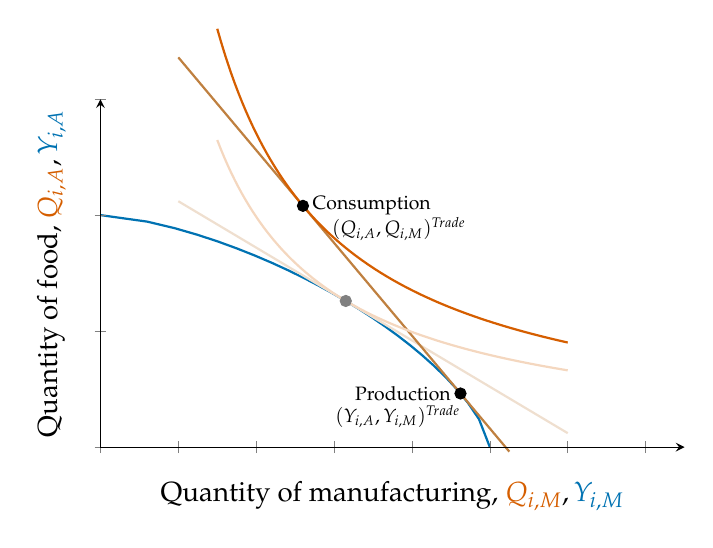
\begin{tikzpicture}
    \pgfmathsetmacro{\beta}{1/3}
    \pgfmathsetmacro{\alpha}{0.5}

    \pgfmathsetmacro{\Zm}{1}
    \pgfmathsetmacro{\K}{1}
    
    \pgfmathsetmacro{\Za}{1}
    \pgfmathsetmacro{\T}{1}

    \pgfmathsetmacro{\Kf}{1}
    \pgfmathsetmacro{\Tf}{15}


    \pgfmathsetmacro{\P}{\Za/\Zm * ((1-\alpha)/\alpha * \T / \K)^(\beta)}   


    \pgfmathsetmacro{\Pw}{\Za/\Zm * ((1-\alpha)/\alpha * ( ( \T + \Tf) / (\K+\Kf ) )^(\beta)}  
    \pgfmathsetmacro{\Qw}{(1-\alpha)/\alpha / \Pw}

    \pgfmathsetmacro{\L}{1}
    \pgfmathsetmacro{\Omega}{(\P *\Zm / \Za)^(1/\beta) * \K / \T}      
    \pgfmathsetmacro{\Ls}{ \Omega / (1+\Omega) * \L}    
    \pgfmathsetmacro{\Ym}{ \Zm * \K^(\beta) * \Ls^(1-\beta) }
    \pgfmathsetmacro{\Ya}{ \Za * \T^(\beta) * (1-\Ls)^(1-\beta) }

    \pgfmathsetmacro{\Omegaw}{(\Pw *\Zm / \Za)^(1/\beta) * \K / \T}      
    \pgfmathsetmacro{\Lsw}{ \Omegaw / (1+\Omegaw) * \L}    
    \pgfmathsetmacro{\Ymw}{ \Zm * \K^(\beta) * \Lsw^(1-\beta) }
    \pgfmathsetmacro{\Yaw}{ \Za * \T^(\beta) * (1-\Lsw)^(1-\beta) }
    \pgfmathsetmacro{\Iw}{ \Pw * \Ymw + \Yaw }
    \pgfmathsetmacro{\Qaw}{(1-\alpha) * \Iw}
    \pgfmathsetmacro{\Qmw}{(\alpha)/\Pw * \Iw}

%    \pgfmathsetmacro{\ws}{ \Pm * \Zm * (1-\beta) * (\K / \Ls )^(\beta) }   
    % Compute utility level
    \pgfmathsetmacro{\U}{(\Ya^(\alpha))*(\Ym^(1 - \alpha))}
    \pgfmathsetmacro{\Uw}{(\Qaw^(\alpha))*(\Qmw^(1 - \alpha))}
    
    % Compute prefactor for indifference curve: Qc = A * Qr^(- (1 - alpha)/alpha)
    \pgfmathsetmacro{\expo}{\alpha/(1 - \alpha)}
    \pgfmathsetmacro{\A}{\U^(1/\alpha)}
    \pgfmathsetmacro{\Aw}{\Uw^(1/\alpha)}
    
    \centering
    \begin{axis}[
        xlabel={Quantity of manufacturing, $\textcolor{red}{Q_{i,M}}, \textcolor{blue}{Y_{i,M}}$},
        ylabel={Quantity of food, $\textcolor{red}{Q_{i,A}}, \textcolor{blue}{Y_{i,A}}$},
        ymin=0, ymax=\L+.5,
        xmin=0, xmax=\L+.5,
        yticklabel=\empty,
        xticklabel=\empty,
        axis lines=left,
        enlargelimits=false,
        clip=false,
        axis on top,
        scaled x ticks=false,
        width=9cm, height=6cm,
        title style={font=\bfseries}
    ]
    
    % PPF: Q_C = (L/a_C) - (a_R/a_C) * Q_R
    \addplot[blue, thick, domain=0:1] ({ \Zm * \K^(\beta) * (\L-x)^(1-\beta)}, {\Za * \T^(\beta) * (x)^(1-\beta)});
    \pgfmathsetmacro{\c}{ \Ym + \P * \Ya }
    \addplot[thick, brown!25, domain=0.2:1.2] { \c - \P*x};

    \pgfmathsetmacro{\cw}{ \Yaw + \Pw * \Ymw }
    \addplot[thick, brown, domain=0.2:1.05] { \cw - \Pw*x};
    % Indifference curve through optimal bundle
    \addplot[thick, red!25, domain=0.3:1.2, samples=100] {\A * x^(-\expo)};
    \addplot[thick, red, domain=0.3:1.2, samples=100] {\Aw * x^(-\expo)};
    
    % Labels
    %\node at (axis cs:3.5,0.03) {\Large $\mathcal{Y}_{US}$};
    %\node at (axis cs:\Lendow/\aR,-.01) {\scriptsize $\frac{L_{US}}{a_{US,R}}$};
    %\node at (axis cs:-.75,\Lendow/\aC) {\scriptsize $\frac{L_{US}}{a_{US,C}}$};
    
    
    % Equilibrium point
    \addplot[only marks, mark=*, color=gray, mark size=2pt] coordinates {(\Ym, \Ya)};
    %\addplot[dashed] coordinates {(\Ya,\Ym) (\Ya,\Ym-.2)};
    %\addplot[dashed] coordinates {(\Ya,\Ym-.2) (\Ya+\P*.2,\Ym-.2)};
    %\node at (axis cs:\Ya + .15,\Ym + 0.1) {\scriptsize $(Q_{i,A},Q_{i,M})$};
    %\node at (axis cs:\Ya+ .1,\Ym-.25) {\scriptsize $1$};
    %\node at (axis cs:\Ya- .05,\Ym-.1) {\scriptsize $\frac{P_A}{P_M}$};
    %\node at (axis cs:\Qr - 2,\Qc + 0.0025) {\scriptsize $\textcolor{blue}{(Y_{US,R},Y_{US,C})}$};
    
    \addplot[only marks, mark=*, color=black, mark size=2pt] coordinates {(\Ymw, \Yaw)};
    \addplot[only marks, mark=*, color=black, mark size=2pt] coordinates {(\Qmw, \Qaw)};
    \node[anchor = west] at (axis cs:\Qmw,\Qaw) {\scriptsize Consumption};
    \node[anchor = west] at (axis cs:\Qmw+0.05,\Qaw-0.1) {\scriptsize $(Q_{i,A},Q_{i,M})^{Trade}$};
    \node[anchor = east] at (axis cs:\Ymw,\Yaw) {\scriptsize Production};
    \node[anchor = east] at (axis cs:\Ymw+0.025,\Yaw-0.1) {\scriptsize $(Y_{i,A},Y_{i,M})^{Trade}$};
    
    
    \end{axis}
    \end{tikzpicture}
    
    \caption{Optimal Consumption and Production Choices for Society as a Whole}
    \label{fig: consumption-trade}
\end{figure}
\end{frame}

\begin{frame}{Trade Equilibrium: Labor Market Shifts}
    \centering
    \begin{tikzpicture}
    
    % Setup axis
    \begin{axis}[
        axis lines=middle,
        xtick=\empty,
        ytick=\empty,
        xmin=0, xmax=2.2,
        ymin=0, ymax=1.2,
        samples=300,
        axis line style={->},
        width=12cm,
        height=8cm,
        domain=0.05:1.05,
        clip=false,
    ]
    \pgfmathsetmacro{\beta}{1/3}
    \pgfmathsetmacro{\alpha}{1/2}

    \pgfmathsetmacro{\Zm}{1}
    \pgfmathsetmacro{\K}{1}
    
    \pgfmathsetmacro{\Za}{1}
    \pgfmathsetmacro{\T}{1}

    \pgfmathsetmacro{\Kf}{1}
    \pgfmathsetmacro{\Tf}{8}


    \pgfmathsetmacro{\P}{\Za/\Zm * ((1-\alpha)/\alpha * \T / \K)^(\beta)}   
    \pgfmathsetmacro{\Pw}{\Za/\Zm * ((1-\alpha)/\alpha * ( ( \T + \Tf) / (\K+\Kf ) )^(\beta)}  

    \pgfmathsetmacro{\L}{2.2}
    \pgfmathsetmacro{\Omega}{(\P *\Zm / \Za)^(1/\beta) * \K / \T}      
    \pgfmathsetmacro{\Ls}{ \Omega / (1+\Omega) * \L}    
    \pgfmathsetmacro{\ws}{ \P * \Zm * (1-\beta) * (\K / \Ls )^(\beta) }

    
    \pgfmathsetmacro{\Omegaw}{(\Pw *\Zm / \Za)^(1/\beta) * \K / \T}      
    \pgfmathsetmacro{\Lsw}{ \Omegaw / (1+\Omegaw) * \L}    
    \pgfmathsetmacro{\wsw}{ \Pw * \Zm * (1-\beta) * (\K / \Lsw )^(\beta) }   
    
    
    \addplot[->] coordinates {(2.2,0) (2.2,1.2)};
    \addplot[->] coordinates {(2.2,0) (0,0)};
    
    
    % Demand in manufacturing (left)
    \addplot[domain=0.2:2.2, thick, red] (x, {\P * \Zm * (1-\beta) * (\K / x)^(\beta)});
    %\node[align=center, anchor=north west, red!70] at (axis cs:0.2,0.65) {\small $P_M \times MPL_{i,M}$};
    \node[black, P] at (axis cs:-0.25,1.15) {\scriptsize $w_i$, \textcolor{red}{$P_M \times MPL_{i,M}$}};
    \node[black] at (axis cs:0,-0.04) {\scriptsize $0~(\bar{L}_i)$};
    
    % Demand in food (right)
    \addplot[domain=0.2:2.2, thick, blue] (2.2-x, {(\Za * (1-\beta) * (\T / x)^(\beta)});
    %\node[align=center, anchor=north east, blue!70] at (axis cs:2.2-0.2,0.65) {\small $P_A \times MPL_{i,A}$};
    \node[black, P] at (axis cs:2.2+0.25,1.15) {\scriptsize $w_i$, \textcolor{blue}{$P_A \times MPL_{i,A}$}};
    \node[black] at (axis cs:2.2,-0.04) {\scriptsize $\bar{L}_i~(0)$};
    
    % Equilibrium point
    \addplot[dashed] coordinates {(0,\ws) (2.2,\ws)};
    \addplot[mark=*, mark size=1.5pt] coordinates {(\Ls,\ws)};
    \addplot[mark=*, mark size=1.5pt] coordinates {(\Ls,{\Pw * \Zm * (1-\beta)*(\K/\Ls)^(\beta)})};
    \addplot[dashed] coordinates {(\Ls,0) (\Ls, {\Pw * \Zm * (1-\beta)*(\K/\Ls)^(\beta)})};
    \node[below] at (axis cs:\Ls,-0.02) {\small $L_M$};
    \node[black, P] at (axis cs:-0.05,\ws) {\scriptsize $w_i^*$};
    \node[black, P] at (axis cs:2.2+0.05,\ws) {\scriptsize $w_i^*$};

    % Bottom left and right axis labels
    %\node[below] at (axis cs:-0.5,-0.02) {\scriptsize $L_M$};
    %\node[below] at (axis cs:0.5,-0.02) {\scriptsize $L - L_M~(= L_F)$};
    
    \end{axis}
    
    \end{tikzpicture}
\end{frame}

\begin{frame}{Trade Equilibrium: Labor Market Shifts}
\addtocounter{framenumber}{-1}
    \centering
    \begin{tikzpicture}
    
    % Setup axis
    \begin{axis}[
        axis lines=middle,
        xtick=\empty,
        ytick=\empty,
        xmin=0, xmax=2.2,
        ymin=0, ymax=1.2,
        samples=300,
        axis line style={->},
        width=12cm,
        height=8cm,
        domain=0.05:1.05,
        clip=false,
    ]
    \pgfmathsetmacro{\beta}{1/3}
    \pgfmathsetmacro{\alpha}{1/2}

    \pgfmathsetmacro{\Zm}{1}
    \pgfmathsetmacro{\K}{1}
    
    \pgfmathsetmacro{\Za}{1}
    \pgfmathsetmacro{\T}{1}

    \pgfmathsetmacro{\Kf}{1}
    \pgfmathsetmacro{\Tf}{8}


    \pgfmathsetmacro{\P}{\Za/\Zm * ((1-\alpha)/\alpha * \T / \K)^(\beta)}   
    \pgfmathsetmacro{\Pw}{\Za/\Zm * ((1-\alpha)/\alpha * ( ( \T + \Tf) / (\K+\Kf ) )^(\beta)}  

    \pgfmathsetmacro{\L}{2.2}
    \pgfmathsetmacro{\Omega}{(\P *\Zm / \Za)^(1/\beta) * \K / \T}      
    \pgfmathsetmacro{\Ls}{ \Omega / (1+\Omega) * \L}    
    \pgfmathsetmacro{\ws}{ \P * \Zm * (1-\beta) * (\K / \Ls )^(\beta) }

    
    \pgfmathsetmacro{\Omegaw}{(\Pw *\Zm / \Za)^(1/\beta) * \K / \T}      
    \pgfmathsetmacro{\Lsw}{ \Omegaw / (1+\Omegaw) * \L}    
    \pgfmathsetmacro{\wsw}{ \Pw * \Zm * (1-\beta) * (\K / \Lsw )^(\beta) }   
    
    
    \addplot[->] coordinates {(2.2,0) (2.2,1.2)};
    \addplot[->] coordinates {(2.2,0) (0,0)};
    
    
    % Demand in manufacturing (left)
    \addplot[domain=0.2:2.2, thick, red!50] (x, {\P * \Zm * (1-\beta) * (\K / x)^(\beta)});
    % Demand in manufacturing (left)
    \addplot[domain=0.7:2.2, thick, red] (x, {\Pw * \Zm * (1-\beta) * (\K / x)^(\beta)});
    %\node[align=center, anchor=north west, red!70] at (axis cs:0.2,0.65) {\small $P_M \times MPL_{i,M}$};
    \node[black, P] at (axis cs:-0.25,1.15) {\scriptsize $w_i$, \textcolor{red}{$P_M \times MPL_{i,M}$}};
    \node[black] at (axis cs:0,-0.04) {\scriptsize $0~(\bar{L}_i)$};
    
    % Demand in food (right)
    \addplot[domain=0.2:2.2, thick, blue] (2.2-x, {(\Za * (1-\beta) * (\T / x)^(\beta)});
    %\node[align=center, anchor=north east, blue!70] at (axis cs:2.2-0.2,0.65) {\small $P_A \times MPL_{i,A}$};
    \node[black, P] at (axis cs:2.2+0.25,1.15) {\scriptsize $w_i$, \textcolor{blue}{$P_A \times MPL_{i,A}$}};
    \node[black] at (axis cs:2.2,-0.04) {\scriptsize $\bar{L}_i~(0)$};
    
    % Equilibrium point
    \addplot[dashed, gray] coordinates {(0,\ws) (2.2,\ws)};
    \addplot[mark=*, gray, mark size=1.5pt] coordinates {(\Ls,\ws)};
    \addplot[mark=*, gray, mark size=1.5pt] coordinates {(\Ls,{\Pw * \Zm * (1-\beta)*(\K/\Ls)^(\beta)})};
    \addplot[dashed, gray] coordinates {(\Ls,0) (\Ls, {\Pw * \Zm * (1-\beta)*(\K/\Ls)^(\beta)})};
    \node[below] at (axis cs:\Ls,-0.02) {\small $L_M$};
    \node[black, P] at (axis cs:-0.05,\ws) {\scriptsize $w_i^*$};
    \node[black, P] at (axis cs:2.2+0.05,\ws) {\scriptsize $w_i^*$};

        \addplot[dashed] coordinates {(0,\wsw) (2.2,\wsw)};
    \addplot[mark=*, black, mark size=1.5pt] coordinates {(\Lsw,\wsw)};
    \addplot[dashed] coordinates {(\Lsw,0) (\Lsw,\wsw)};
    \node[below] at (axis cs:\Lsw,-0.02) {\small $(L_M)^{Trade}$};
    \node[black, P] at (axis cs:-0.12,\wsw) {\scriptsize $(w_i^*)^{Trade}$};
    \node[black, P] at (axis cs:2.2+0.12,\wsw) {\scriptsize $(w_i^*)^{Trade}$};

    % Bottom left and right axis labels
    %\node[below] at (axis cs:-0.5,-0.02) {\scriptsize $L_M$};
    %\node[below] at (axis cs:0.5,-0.02) {\scriptsize $L - L_M~(= L_F)$};
    
    \end{axis}
    
    \end{tikzpicture}
\end{frame}


\end{document}
